\documentclass[11pt,letterpaper]{article}
\usepackage{fontspec}
\setmainfont{texgyrepagella}[Extension=.otf,UprightFont=*-regular,BoldFont=*-bold,ItalicFont=*-italic,BoldItalicFont=*-bolditalic]
\usepackage[bidi=default]{babel}
\babelprovide[import,main]{spanish}
\babelprovide[import]{hebrew}
\babelprovide[import]{ancientgreek}
\babelfont[hebrew]{rm}[Path=fonts/,BoldFont=NotoHebrewSerif-700.ttf,Scale=0.95]{NotoHebrewSerif-400.ttf}
\babelfont[ancientgreek]{rm}[Path=fonts/]{GFSPorson.otf}
\newcommand{\heb}[1]{\mbox{\foreignlanguage{hebrew}{#1}}}
\newcommand{\grc}[1]{\foreignlanguage{ancientgreek}{#1}}
\newcommand{\hebverso}[1]{\par\smallskip{\centering\begin{otherlanguage}{hebrew}\large #1\end{otherlanguage}\par}\smallskip}
\newcommand{\SENOR}{\textsc{Señor}}
\usepackage[margin=2.5cm,headheight=14pt]{geometry}
\usepackage{microtype,ragged2e,booktabs,graphicx,xcolor,csquotes,array}
\usepackage[hidelinks]{hyperref}\usepackage{xurl}\urlstyle{same}
\usepackage[most]{tcolorbox}
\usepackage{tikz}\usetikzlibrary{arrows.meta,positioning,calc,decorations.pathreplacing,shapes.geometric}
\usepackage{titlesec,fancyhdr,needspace}
\definecolor{tierraroja}{RGB}{122,40,18}\definecolor{caferojizo}{RGB}{58,18,8}
\definecolor{mostaza}{RGB}{214,160,58}\definecolor{papiro}{RGB}{243,228,192}\definecolor{sepia}{RGB}{98,66,44}
\definecolor{oliva}{RGB}{92,98,48}
\titleformat{\section}{\Large\bfseries\color{tierraroja}}{\thesection.}{0.6em}{}
\titleformat{\subsection}{\large\bfseries\color{caferojizo}}{\thesubsection}{0.6em}{}
\pagestyle{fancy}\fancyhf{}
\fancyhead[L]{\foreignlanguage{spanish}{\small\itshape\color{sepia}Shavuot}}\fancyhead[R]{\foreignlanguage{spanish}{\small\color{sepia}\thepage}}
\renewcommand{\headrulewidth}{0.4pt}
\setlength{\parindent}{1.27cm}\linespread{1.15}\setlength{\emergencystretch}{3em}
\newtcolorbox{cita}[1][]{enhanced,unbreakable,colback=tierraroja!5!white,colframe=tierraroja,boxrule=0pt,leftrule=2.5pt,arc=0pt,
  left=8pt,right=8pt,top=5pt,bottom=5pt,before skip=8pt,after skip=8pt,fontupper=\itshape,#1}
\newcommand{\fuente}[1]{\par\hfill{\upshape\bfseries\small\textcolor{tierraroja}{#1}}}
\newtcolorbox{nota}[1][]{enhanced,unbreakable,colback=mostaza!10,colframe=mostaza!85!tierraroja,boxrule=0.6pt,arc=2pt,
  fonttitle=\bfseries\small,coltitle=caferojizo,colbacktitle=mostaza!30,fontupper=\small,title={#1}}
\newtcolorbox{filologia}[1][]{enhanced,unbreakable,colback=white,colframe=tierraroja!45,boxrule=0.5pt,arc=2pt,
  fonttitle=\bfseries\small,coltitle=white,colbacktitle=tierraroja!80,fontupper=\small,title={Filología: #1}}
\newcommand{\refapa}[1]{\par{\RaggedRight\hangindent=1.27cm\hangafter=1\noindent #1\par}\vspace{4pt}}
\newcommand{\destacar}[1]{\textbf{\textcolor{tierraroja}{#1}}}
\newcolumntype{L}[1]{>{\RaggedRight\arraybackslash}p{#1}}

\title{\color{tierraroja}\bfseries Shavuot: la fiesta de las Semanas (Pentecostés)\\[4pt]\large\color{sepia}\mdseries ``Hasta el día siguiente del séptimo día de reposo contaréis cincuenta días'' (Lv 23:16)}
\author{}\date{}
\begin{document}
\maketitle\thispagestyle{empty}

\begin{abstract}\noindent
Shavuot es la única fiesta de Levítico 23 que no tiene fecha: se llega a ella contando. Desde el día en que se mecía el \emph{ómer} de la cebada, Israel debía contar ``siete semanas cumplidas'' (\emph{sheva shabatot temimot}) hasta el día cincuenta, y entonces presentar una ofrenda nueva de trigo: dos panes cocidos con levadura, la única ofrenda leudada del calendario. La Torá la llama fiesta de la siega (Éx 23:16), fiesta de las semanas (Éx 34:22; Dt 16:10) y día de las primicias (Nm 28:26); el griego del Segundo Templo la llamó \emph{pentēkostē}, ``el quincuagésimo'' (Tob 2:1; 2~Mac 12:32; Hch 2:1). El estudio sigue el método de la serie: lectura histórica (la siega del trigo, Rut, la peregrinación, la diáspora reunida en Jerusalén), filológica (\emph{shavúa}, \emph{temimot}, \emph{bikurim}, \emph{jamets}, \emph{peá}, \emph{léqet}, las ``voces'' y el fuego del Sinaí, las lenguas de Hechos 2, las lluvias \emph{yoré} y \emph{malqosh}), textual (el cómputo de Lv 23:15--16, Joel 2:23 en el texto masorético y en la Septuaginta) y literaria (los paralelos Sinaí--Hechos 2, Números 11, Babel, Jeremías 31 y 2~Corintios 3). Expone la lectura de la serie, que ve en Shavuot el memorial del Sinaí y la figura del derramamiento del Espíritu, en los dos panes con levadura a los pueblos aún con pecado considerados para la redención, y en las lluvias de Joel 2:23 las etapas de la obra del Espíritu. Donde el texto bíblico no dice lo que la tradición o la tipología le atribuyen, lo señalo con una precisión.
\par\smallskip\noindent\textbf{Palabras clave:} Shavuot, Pentecostés, fiesta de las Semanas, Levítico 23, dos panes, Sinaí, Hechos 2, Joel 2:23, lluvia temprana y tardía.\end{abstract}

\begin{nota}[Nota sobre el texto]
Las citas bíblicas son de la Reina-Valera 1960 (RVR1960). Donde esta escribe ``Jehová'', aquí se escribe \SENOR, que traduce el tetragrama \heb{יהוה}. El hebreo sigue la \emph{Biblia Hebraica Stuttgartensia} (BHS), sin acentos masoréticos; el griego, NA28 y la Septuaginta de Rahlfs-Hanhart. Cuando la numeración hebrea difiere de la española se da entre corchetes: Joel 2:28--32 [3:1--5]. Tobías y 2~Macabeos son libros deuterocanónicos: se citan como testimonio histórico del judaísmo del Segundo Templo, no como Escritura de la serie. Las fuentes judías posteriores (Misná, Talmud, \emph{midrash}, liturgia) se citan desde Sefaria y la edición de Danby (1933), y se marcan como tradición. Este estudio supone el de las Primicias (estudio~3), donde se discute el ``día siguiente del sábado'' (Lv 23:11, 15). El marco de la serie se toma del documento de referencia (lecciones 6--11) y de mi presentación anterior sobre Pentecostés, cuyos temas (el ciclo agrícola, la cuenta del \emph{ómer}, el clima, Joel 2:23, el pacto matrimonial, las arras del Espíritu y las tres trompetas) se integran en las secciones correspondientes.
\end{nota}

%===================================================================
\section{Introducción: una fiesta a la que se llega contando}

Pésaj tiene fecha: el día catorce del mes primero, entre las dos tardes. Matsot también, del quince al veintiuno. Yom Teruá, Yom Kipur y Sukkot llevan su día y su mes escritos en Levítico 23. Shavuot no. En lugar de ``en el mes tercero, a los seis días'', el texto dice ``contaréis'', e Israel llega a esta fiesta caminando un día detrás de otro desde la primera gavilla de la cebada hasta el trigo maduro, cuarenta y nueve días que terminan en un día cincuenta. De ahí que la pregunta sea doble: ¿qué se cuenta, y hacia qué?

La Torá responde primero con el campo. Las siete semanas son las de la siega del grano, desde que ``comenzare a meterse la hoz en las mieses'' (Dt 16:9) hasta las ``primicias de la siega del trigo'' (Éx 34:22). Al final de la cuenta Israel ya no lleva espigas sueltas sino pan hecho: dos panes de flor de harina, cocidos con levadura, mecidos ante el \SENOR{} como primicias (Lv 23:17). Y en el mismo párrafo la ley se vuelve al pobre y al extranjero, porque el rincón del campo y las espigas caídas no pertenecen al dueño (Lv 23:22).

El Nuevo Testamento responde con un acontecimiento. ``Cuando llegó el día de Pentecostés'', el día cincuenta, los discípulos estaban reunidos en Jerusalén; vino del cielo un estruendo como de viento, aparecieron lenguas como de fuego, y fueron llenos del Espíritu Santo (Hch 2:1--4). Pedro explica lo ocurrido con el profeta Joel: ``derramaré mi Espíritu sobre toda carne'' (Hch 2:17; Jl 2:28 [3:1]).

Entre el campo y Hechos 2 está el Sinaí. Israel llegó al monte ``en el mes tercero'' (Éx 19:1), el mes de la siega del trigo, y allí oyó la voz de Dios en medio del fuego. La serie toma ese hecho como el hito que Shavuot conmemora: \destacar{la fiesta de la siega es el memorial de la manifestación de Dios en el Sinaí y de la entrega de la Ley, y la figura del derramamiento del Espíritu}. Quiero mostrar que esa tesis tiene apoyo real en la Escritura y en el judaísmo del Segundo Templo, y precisar dónde ese apoyo es explícito y dónde es lectura posterior.

\begin{center}
% === Esquema estándar de la serie: el ciclo de Levítico 23 ===
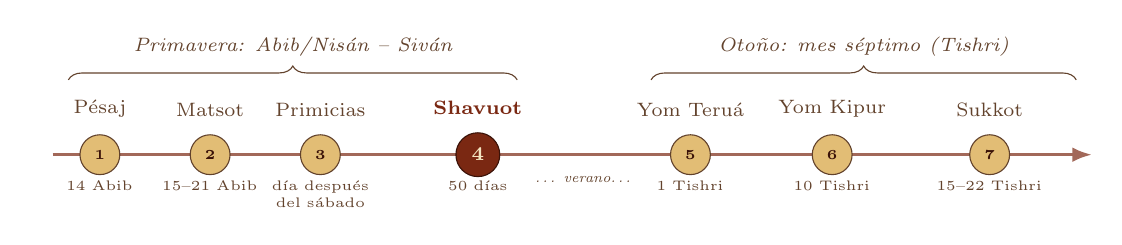
\begin{tikzpicture}[x=1cm,y=1cm,font=\scriptsize]
 \def\fiestaactual{4}
 \draw[line width=1.2pt,tierraroja!70,-{Latex[length=2.5mm]}] (0,0) -- (13.2,0);
 \draw[decorate,decoration={brace,amplitude=5pt},sepia] (0.2,0.95) -- (5.9,0.95) node[midway,above=5pt,font=\scriptsize\itshape]{Primavera: Abib/Nisán -- Siván};
 \draw[decorate,decoration={brace,amplitude=5pt},sepia] (7.6,0.95) -- (13.0,0.95) node[midway,above=5pt,font=\scriptsize\itshape]{Otoño: mes séptimo (Tishri)};
 \foreach \n/\x/\t/\d in {1/0.6/Pésaj/{14 Abib},2/2.0/Matsot/{15--21 Abib},3/3.4/Primicias/{día después del sábado},4/5.4/Shavuot/{50 días},5/8.1/Yom Teruá/{1 Tishri},6/9.9/Yom Kipur/{10 Tishri},7/11.9/Sukkot/{15--22 Tishri}}{
   \ifnum\n=\fiestaactual
     \node[circle,fill=tierraroja,draw=caferojizo,minimum size=5.5mm,text=papiro,font=\scriptsize\bfseries] at (\x,0) {\n};
     \node[above=3pt,font=\scriptsize\bfseries,text=tierraroja] at (\x,0.28) {\t};
   \else
     \node[circle,fill=mostaza!70,draw=sepia,minimum size=4.5mm,text=caferojizo,font=\tiny\bfseries] at (\x,0) {\n};
     \node[above=3pt,text=sepia] at (\x,0.25) {\t};
   \fi
   \node[below=6pt,text width=1.6cm,align=center,font=\tiny,text=sepia] at (\x,0) {\d};}
 \node[font=\tiny\itshape,text=sepia] at (6.75,-0.32) {\ldots\ verano\ldots};
\end{tikzpicture}\par
{\footnotesize\color{sepia}\textit{Figura 1.} El ciclo de Levítico 23: Shavuot cierra el grupo de primavera. \textit{Nota.} Elaboración propia; esquema común de la serie.}
\end{center}

Pésaj, Matsot y la gavilla de las Primicias se concentran en una semana; Shavuot viene siete semanas después, unida a ellas por la cuenta, y cierra el grupo de primavera. En el esquema de la serie, la primavera mira hacia lo ya ocurrido en la historia de la salvación (la cruz, la salida del pecado, la resurrección y el don del Espíritu), y el otoño hacia lo que falta.

El recorrido sigue el orden habitual de la serie: el texto (§2), las lecturas histórica, filológica, textual y literaria (§3--6), la lectura de la serie (§7), Jesús y los apóstoles (§8), la tradición judía (§9), la discusión de interpretaciones (§10), la síntesis (§11) y las preguntas (§12).

%===================================================================
\section{El texto: siete semanas, un día cincuenta}

\subsection{Texto ancla: Levítico 23:15--17}

El párrafo de Shavuot sigue sin pausa al de la gavilla de las primicias, con el mismo sujeto (``vosotros'') y el mismo punto de partida (``el día que sigue al día de reposo''): la cebada abre la cuenta y el trigo la cierra.

\needspace{5\baselineskip}\hebverso{וּסְפַרְתֶּם לָכֶם מִמָּחֳרַת הַשַּׁבָּת מִיּוֹם הֲבִיאֲכֶם אֶת־עֹמֶר הַתְּנוּפָה שֶׁבַע שַׁבָּתוֹת תְּמִימֹת תִּהְיֶינָה \\ עַד מִמָּחֳרַת הַשַּׁבָּת הַשְּׁבִיעִת תִּסְפְּרוּ חֲמִשִּׁים יוֹם וְהִקְרַבְתֶּם מִנְחָה חֲדָשָׁה לַיהוָה}
\begin{cita}Y contaréis desde el día que sigue al día de reposo, desde el día en que ofrecisteis la gavilla de la ofrenda mecida; siete semanas cumplidas serán. Hasta el día siguiente del séptimo día de reposo contaréis cincuenta días; entonces ofreceréis el nuevo grano a \SENOR. De vuestras habitaciones traeréis dos panes para ofrenda mecida, que serán de dos décimas de efa de flor de harina, cocidos con levadura, como primicias para \SENOR.\fuente{(Lv 23:15--17)}\end{cita}

Tres verbos ordenan el párrafo: \emph{contar} (\heb{וּסְפַרְתֶּם}, \emph{usfartem}), \emph{traer} (\heb{תָּבִיאוּ}, \emph{taví'u}) y \emph{ofrecer} (\heb{וְהִקְרַבְתֶּם}, \emph{vehiqravtem}). La cuenta tiene dos extremos marcados con la misma expresión, ``el día siguiente del sábado'' (\heb{מִמָּחֳרַת הַשַּׁבָּת}), y se formula de dos maneras, ``siete \emph{shabatot} cumplidas'' y ``cincuenta días''. La ofrenda recibe un nombre que no había aparecido antes, \heb{מִנְחָה חֲדָשָׁה} (\emph{minjá jadashá}), ``ofrenda nueva'', que la RVR1960 traduce ``el nuevo grano'' porque es la primera ofrenda del templo hecha con el grano del año.

\needspace{5\baselineskip}\hebverso{מִמּוֹשְׁבֹתֵיכֶם תָּבִיאוּ לֶחֶם תְּנוּפָה שְׁתַּיִם שְׁנֵי עֶשְׂרֹנִים סֹלֶת תִּהְיֶינָה חָמֵץ תֵּאָפֶינָה בִּכּוּרִים לַיהוָה}

El versículo 17 reúne cuatro rasgos que ninguna otra ofrenda del calendario comparte. Los panes vienen ``de vuestras habitaciones'' (\heb{מִמּוֹשְׁבֹתֵיכֶם}), del pan de las casas y no de la cocina del santuario. Son dos. Son de flor de harina de trigo, el grano de esta siega (Éx 34:22). Y son \heb{חָמֵץ} (\emph{jamets}), ``leudados'', la misma palabra que durante Matsot no podía aparecer en ninguna casa de Israel (Éx 12:15, 19; 13:7).

\subsection{Los sacrificios y la ley del campo (Lv 23:18--22)}

Con los panes se ofrecen siete corderos de un año, un becerro y dos carneros en holocausto, un macho cabrío por el pecado y dos corderos en sacrificio de paz (vv. 18--19). El sacerdote mece los dos corderos de paz junto con ``el pan de las primicias'', y todo queda para él como ``cosa sagrada'' (v. 20). El día es \emph{mikrá kódesh}, santa convocación, sin ``trabajo de siervos'', ``estatuto perpetuo en dondequiera que habitéis por vuestras generaciones'' (v. 21). Antes de pasar al mes séptimo, el texto agrega una ley que ya no pertenece a la liturgia:

\needspace{5\baselineskip}\hebverso{וּבְקֻצְרְכֶם אֶת־קְצִיר אַרְצְכֶם לֹא־תְכַלֶּה פְּאַת שָׂדְךָ בְּקֻצְרֶךָ \\ וְלֶקֶט קְצִירְךָ לֹא תְלַקֵּט לֶעָנִי וְלַגֵּר תַּעֲזֹב אֹתָם אֲנִי יְהוָה אֱלֹהֵיכֶם}
\begin{cita}Cuando segareis la mies de vuestra tierra, no segaréis hasta el último rincón de ella, ni espigarás tu siega; para el pobre y para el extranjero la dejarás. Yo \SENOR{} vuestro Dios.\fuente{(Lv 23:22)}\end{cita}

La ley repite casi palabra por palabra Lv 19:9--10, y su lugar aquí hace que la fiesta de la siega termine en el borde del campo y no en el altar. La \emph{peá} (\heb{פֵּאָה}, ``rincón, borde'') y el \emph{léqet} (\heb{לֶקֶט}, ``espigueo'') son la parte de la cosecha que el dueño no recoge, porque Dios la asignó al pobre (\heb{עָנִי}) y al extranjero residente (\heb{גֵּר}).

\subsection{Los otros textos legislativos}

La fiesta aparece en los cuatro calendarios de la Torá y cada uno le da un nombre y un énfasis.

\begin{cita}También la fiesta de la siega, los primeros frutos de tus labores, que hubieres sembrado en el campo, y la fiesta de la cosecha a la salida del año, cuando hayas recogido los frutos de tus labores del campo.\fuente{(Éx 23:16)}\end{cita}

\begin{cita}También celebrarás la fiesta de las semanas, la de las primicias de la siega del trigo, y la fiesta de la cosecha a la salida del año.\fuente{(Éx 34:22)}\end{cita}

\begin{cita}Además, el día de las primicias, cuando presentéis ofrenda nueva a \SENOR{} en vuestras semanas, tendréis santa convocación; ninguna obra de siervos haréis.\fuente{(Nm 28:26)}\end{cita}

\needspace{5\baselineskip}\hebverso{וְשָׂמַחְתָּ לִפְנֵי יְהוָה אֱלֹהֶיךָ אַתָּה וּבִנְךָ וּבִתֶּךָ וְעַבְדְּךָ וַאֲמָתֶךָ \\ וְהַלֵּוִי אֲשֶׁר בִּשְׁעָרֶיךָ וְהַגֵּר וְהַיָּתוֹם וְהָאַלְמָנָה אֲשֶׁר בְּקִרְבֶּךָ}
\begin{cita}Siete semanas contarás; desde que comenzare a meterse la hoz en las mieses comenzarás a contar las siete semanas. Y harás la fiesta solemne de las semanas a \SENOR{} tu Dios; de la abundancia voluntaria de tu mano será lo que dieres, según \SENOR{} tu Dios te hubiere bendecido. Y te alegrarás delante de \SENOR{} tu Dios, tú, tu hijo, tu hija, tu siervo, tu sierva, el levita que habitare en tus ciudades, y el extranjero, el huérfano y la viuda que estuvieren en medio de ti, en el lugar que \SENOR{} tu Dios hubiere escogido para poner allí su nombre. Y acuérdate de que fuiste siervo en Egipto; por tanto, guardarás y cumplirás estos estatutos.\fuente{(Dt 16:9--12)}\end{cita}

Deuteronomio no menciona los dos panes ni los sacrificios; habla de alegría, de generosidad ``según te hubiere bendecido'' y de memoria. La lista de los que se alegran forma dos grupos (Tigay, 1996): la casa (hijo, hija, siervo, sierva) y los que no tienen tierra propia (levita, extranjero, huérfano, viuda). La razón que da el texto es histórica, ``acuérdate de que fuiste siervo en Egipto'' (v. 12), de modo que la fiesta de la abundancia es también la del esclavo que recuerda.

Deuteronomio cierra el calendario con la regla de las tres peregrinaciones: ``Tres veces cada año aparecerá todo varón tuyo delante de \SENOR{} tu Dios en el lugar que él escogiere\ldots{} y ninguno se presentará delante de \SENOR{} con las manos vacías; cada uno con la ofrenda de su mano, conforme a la bendición que \SENOR{} tu Dios te hubiere dado'' (Dt 16:16--17). En mi presentación anterior cité aquí el comentario judío \emph{Minjá Belulá} (Abraham Menajem Rapa Porto, Verona, 1594), según el cual las peregrinaciones fomentaban el amor y la hermandad entre los israelitas. Es una lectura tradicional, coherente con la alegría compartida de Dt 16:11.

\begin{center}\small\renewcommand{\arraystretch}{1.22}
\begin{tabular}{@{}L{2.2cm}L{3.6cm}L{9.6cm}@{}}
\toprule
\textbf{Texto} & \textbf{Nombre} & \textbf{Lo que añade} \\ \midrule
Éx 23:14--17 & \heb{חַג הַקָּצִיר} \emph{jag haqatsir}, ``fiesta de la siega'' & Una de las tres fiestas de peregrinación (\emph{shalosh regalim}): ``tres veces en el año se presentará todo varón'' (v. 17). Primicias ``de tus labores''. \\
Éx 34:22--23 & \heb{חַג שָׁבֻעֹת} \emph{jag shavuot}, ``fiesta de las semanas'' & Primer uso del nombre ``semanas''; precisa el grano: \heb{בִּכּוּרֵי קְצִיר חִטִּים} (\emph{bikuré qetsir jitim}), ``primicias de la siega del trigo''. \\
Lv 23:15--22 & sin nombre propio; ``ofrenda nueva'' & La cuenta de siete semanas \emph{temimot} y cincuenta días desde el \emph{ómer}; dos panes leudados; sacrificios; santa convocación; \emph{peá} y \emph{léqet} para el pobre y el extranjero. \\
Nm 28:26--31 & \heb{יוֹם הַבִּכּוּרִים} \emph{yom habikurim}, ``día de las primicias'' & ``En vuestras semanas'' (\heb{בְּשָׁבֻעֹתֵיכֶם}); sacrificios adicionales del día: dos becerros, un carnero, siete corderos y un macho cabrío. \\
Dt 16:9--12, 16 & \heb{חַג שָׁבֻעוֹת} & La cuenta empieza ``desde que comenzare a meterse la hoz''; ofrenda voluntaria según la bendición; alegría inclusiva; ``acuérdate de que fuiste siervo''; en el lugar escogido. \\
2~Cr 8:13 & ``fiesta de las semanas'' & Salomón ofrece en las tres fiestas anuales: Ázimos, Semanas y Tabernáculos. \\
Tob 2:1; 2~Mac 12:31--32 & \grc{πεντηκοστή} \emph{pentēkostē} & Deuterocanónicos: primer uso del nombre griego ``Pentecostés'' para la fiesta. \\
Hch 2:1; 20:16; 1~Co 16:8 & \grc{ἡ ἡμέρα τῆς πεντηκοστῆς} & El día del derramamiento del Espíritu; Pablo organiza sus viajes en torno a la fiesta. \\
\bottomrule
\end{tabular}\par
{\footnotesize\color{sepia}\textit{Tabla 1.} Tabla sinóptica de los textos de Shavuot. \textit{Nota.} Elaboración propia con la BHS, la LXX y NA28. Tobías y 2~Macabeos son deuterocanónicos.}
\end{center}

\begin{nota}[Precisión]
Los sacrificios de Lv 23:18 (un becerro y dos carneros) y los de Nm 28:27 (dos becerros y un carnero) no coinciden. La tradición rabínica los suma como dos series distintas: los de Levítico acompañan a los panes y los de Números son la ofrenda adicional del día (b. Menajot 45b; cf. Josefo, \emph{Ant.} 3.253, que suma ambas series). Muchos comentaristas modernos ven aquí dos tradiciones sacerdotales que el texto final yuxtapone (Milgrom, 2001; Levine, 1989). El texto no resuelve la diferencia.
\end{nota}

\subsection{Cuarenta y nueve más uno}

La cuenta puede dibujarse como una cuadrícula de siete por siete. El primer día es el del \emph{ómer}, el último de cada fila cierra una semana, y el día cincuenta queda fuera de la cuadrícula, como un día nuevo.

\begin{center}
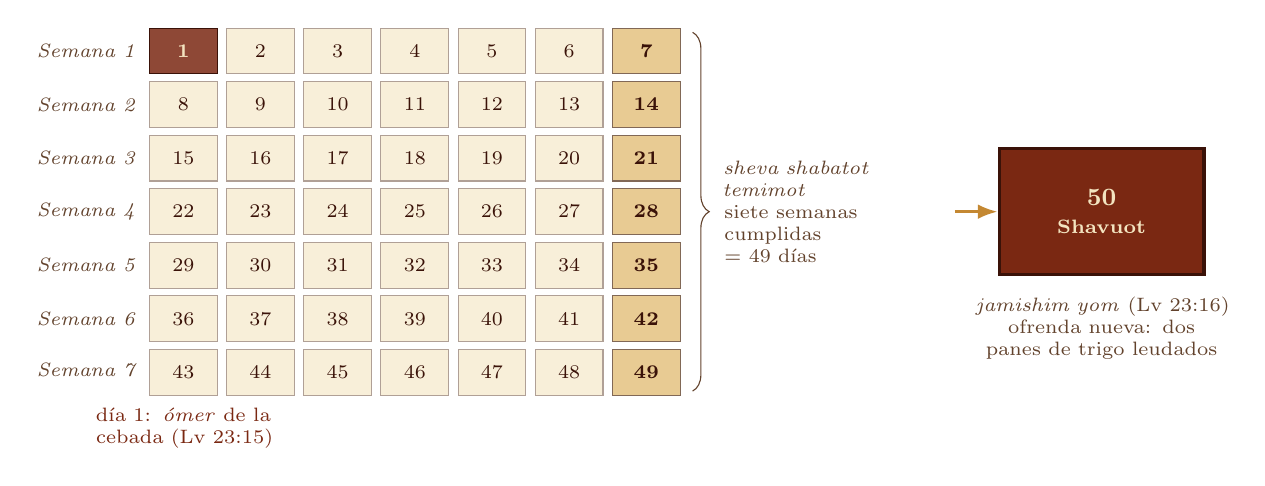
\begin{tikzpicture}[x=0.98cm,y=0.68cm]
 \foreach \w in {1,...,7}{
  \node[font=\scriptsize\itshape,text=sepia,anchor=east] at (0.5,-\w) {Semana \w};
  \foreach \d in {1,...,7}{
    \pgfmathtruncatemacro{\n}{(\w-1)*7+\d}
    \ifnum\n=1
      \node[draw=caferojizo,fill=tierraroja!85,text=papiro,minimum width=0.86cm,minimum height=0.58cm,font=\scriptsize\bfseries] at (\d,-\w) {\n};
    \else\ifnum\d=7
      \node[draw=sepia!80,fill=mostaza!55,text=caferojizo,minimum width=0.86cm,minimum height=0.58cm,font=\scriptsize\bfseries] at (\d,-\w) {\n};
    \else
      \node[draw=sepia!50,fill=papiro!60,text=caferojizo,minimum width=0.86cm,minimum height=0.58cm,font=\scriptsize] at (\d,-\w) {\n};
    \fi\fi}}
 \draw[decorate,decoration={brace,amplitude=6pt},sepia] (7.6,-0.65) -- (7.6,-7.35) node[midway,right=8pt,font=\scriptsize,text width=2.6cm,align=left]{\emph{sheva shabatot temimot}\\ siete semanas cumplidas\\ = 49 días};
 \node[draw=caferojizo,line width=1.2pt,fill=tierraroja,text=papiro,minimum width=2.6cm,minimum height=1.6cm,align=center,font=\small\bfseries] (s) at (12.9,-4) {50\\[-1pt]{\scriptsize Shavuot}};
 \draw[-{Latex[length=2.5mm]},line width=1pt,mostaza!80!tierraroja] (11.0,-4) -- (s.west);
 \node[below=4pt of s,font=\scriptsize,text width=3.2cm,align=center,text=sepia] {\emph{jamishim yom} (Lv 23:16)\\ ofrenda nueva: dos panes de trigo leudados};
 \node[font=\scriptsize,text width=3.2cm,align=center,text=tierraroja] at (1,-8.05) {día 1: \emph{ómer} de la cebada (Lv 23:15)};
\end{tikzpicture}\par
{\footnotesize\color{sepia}\textit{Figura 2.} La cuenta de Lv 23:15--16: siete semanas cumplidas y el día cincuenta. \textit{Nota.} Elaboración propia. El día del \emph{ómer} se cuenta como día 1, según la práctica antigua; el estudio~3 discute desde cuándo se cuenta.}
\end{center}

La cifra cincuenta tiene un eco directo en el Jubileo. Levítico 25 usa el mismo esquema para los años: ``Y contarás siete semanas de años, siete veces siete años, de modo que los días de las siete semanas de años vendrán a serte cuarenta y nueve años'' (Lv 25:8), y el año cincuenta será santo, con libertad proclamada en la tierra (25:10). Shavuot sería así un jubileo pequeño, contado en días. La serie dedica un estudio aparte al Jubileo; baste señalar que ambas instituciones comparten el verbo \emph{contar} (\heb{סָפַר}), la estructura siete por siete y el cincuenta como día o año nuevo.

%===================================================================
\section{Lectura histórica}

\subsection{La siega del trigo en la tierra de Israel}

En la tierra de Israel el año agrícola empieza en otoño. Las primeras lluvias (\emph{yoré}) ablandan la tierra en octubre y noviembre y hacen posible arar y sembrar; las lluvias de invierno hacen crecer el grano; las lluvias tardías (\emph{malqosh}) de marzo y abril lo llenan antes de madurar. La cebada madura primero, hacia marzo y abril, y el trigo unas semanas después, entre mayo y junio. Éxodo registra esa diferencia al contar la séptima plaga: ``El lino, pues, y la cebada fueron destrozados, porque la cebada estaba ya espigada, y el lino en caña. Mas el trigo y el centeno no fueron destrozados, porque eran tardíos'' (Éx 9:31--32). Entre la cebada de Pésaj y el trigo de Shavuot caben las siete semanas de la siega.

El llamado \emph{Calendario de Gézer}, una tablilla de piedra caliza del siglo \textsc{x} a.\,e.\,c., enumera los meses por sus faenas. Dos líneas seguidas dicen \emph{yeraj qetsir se'orim}, ``mes de la siega de la cebada'', y \emph{yeraj qetsir vekhol}, ``mes de la siega y la medida'' (o ``y el acopio'') del grano (Borowski, 1987). Es la secuencia de Levítico 23 vista desde el campo: primero la cebada, después el resto de la siega.

\begin{center}
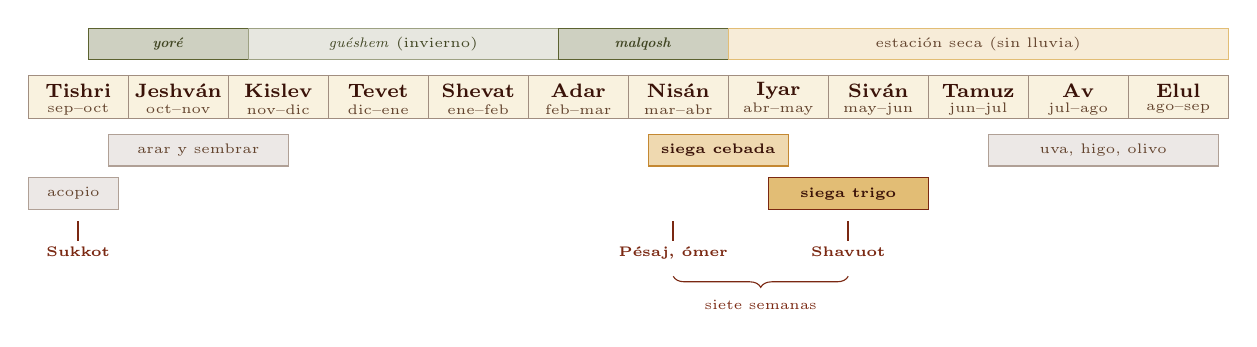
\begin{tikzpicture}[x=1.27cm,y=1cm,font=\scriptsize]
 \foreach \i/\m/\g in {0/Tishri/sep--oct,1/Jeshván/oct--nov,2/Kislev/nov--dic,3/Tevet/dic--ene,4/Shevat/ene--feb,5/Adar/feb--mar,6/Nisán/mar--abr,7/Iyar/abr--may,8/Siván/may--jun,9/Tamuz/jun--jul,10/Av/jul--ago,11/Elul/ago--sep}{
   \draw[sepia!60,fill=papiro!50] (\i,0) rectangle (\i+1,0.55);
   \node[font=\scriptsize\bfseries,text=caferojizo] at (\i+0.5,0.36) {\m};
   \node[font=\tiny,text=sepia] at (\i+0.5,0.12) {\g};}
 % lluvias
 \fill[oliva!30,draw=oliva] (0.6,0.75) rectangle (2.2,1.15); \node[font=\tiny\bfseries,text=oliva!70!black] at (1.4,0.95) {\emph{yoré}};
 \fill[oliva!15,draw=oliva!60] (2.2,0.75) rectangle (5.3,1.15); \node[font=\tiny,text=oliva!70!black] at (3.75,0.95) {\emph{guéshem} (invierno)};
 \fill[oliva!30,draw=oliva] (5.3,0.75) rectangle (7.0,1.15); \node[font=\tiny\bfseries,text=oliva!70!black] at (6.15,0.95) {\emph{malqosh}};
 \fill[mostaza!20,draw=mostaza!70] (7.0,0.75) rectangle (12,1.15); \node[font=\tiny,text=sepia] at (9.5,0.95) {estación seca (sin lluvia)};
 % faenas
 \fill[sepia!12,draw=sepia!50] (0.8,-0.2) rectangle (2.6,-0.6); \node[font=\tiny,text=sepia] at (1.7,-0.4) {arar y sembrar};
 \fill[mostaza!40,draw=mostaza!80!tierraroja] (6.2,-0.2) rectangle (7.6,-0.6); \node[font=\tiny\bfseries,text=caferojizo] at (6.9,-0.4) {siega cebada};
 \fill[mostaza!70,draw=tierraroja] (7.4,-0.75) rectangle (9.0,-1.15); \node[font=\tiny\bfseries,text=caferojizo] at (8.2,-0.95) {siega trigo};
 \fill[sepia!12,draw=sepia!50] (9.6,-0.2) rectangle (11.9,-0.6); \node[font=\tiny,text=sepia] at (10.75,-0.4) {uva, higo, olivo};
 \fill[sepia!12,draw=sepia!50] (0,-0.75) rectangle (0.9,-1.15); \node[font=\tiny,text=sepia] at (0.45,-0.95) {acopio};
 % fiestas
 \foreach \x/\t in {6.45/{Pésaj, ómer},8.2/{Shavuot},0.5/{Sukkot}}{
   \draw[tierraroja,line width=0.8pt] (\x,-1.3) -- (\x,-1.55);
   \node[below,font=\tiny\bfseries,text=tierraroja] at (\x,-1.5) {\t};}
 \draw[decorate,decoration={brace,amplitude=4pt,mirror},tierraroja] (6.45,-2.0) -- (8.2,-2.0) node[midway,below=5pt,font=\tiny,text=tierraroja]{siete semanas};
\end{tikzpicture}\par
{\footnotesize\color{sepia}\textit{Figura 3.} Calendario agrícola de la tierra de Israel: lluvia temprana (\emph{yoré}), lluvias de invierno, lluvia tardía (\emph{malqosh}), siegas y fiestas. \textit{Nota.} Elaboración propia a partir de Borowski (1987) y Dt 11:14; las fechas son aproximadas y varían cada año.}
\end{center}

La figura muestra un dato que habrá que recordar al llegar a las lluvias de Joel (§7): Shavuot cae al comienzo de la estación seca, de modo que una tormenta en la siega del trigo era un prodigio y una señal de juicio. Samuel la usa así ante el pueblo que pidió rey: ``¿No es ahora la siega del trigo? Yo clamaré a \SENOR, y él dará truenos y lluvias'' (1~S 12:17). Los ``truenos'' de ese texto son \heb{קֹלוֹת} (\emph{qolot}), ``voces'', la misma palabra de Éx 19:16. Proverbios usa la imagen para lo que está fuera de lugar: ``Como no conviene la nieve en el verano, ni la lluvia en la siega, así no conviene al necio la honra'' (Pr 26:1).

\subsection{Rut: la fiesta en una historia}

La Biblia no narra ninguna celebración de Shavuot, pero sí narra su estación. El libro de Rut transcurre entre las dos siegas: Noemí y Rut llegan a Belén ``al comienzo de la siega de la cebada'' (Rt 1:22), y Rut espiga en los campos de Booz ``hasta que se acabó la siega de la cebada y la de trigo'' (2:23), justamente las siete semanas de la cuenta.

\needspace{5\baselineskip}\hebverso{וַתֵּלֶךְ וַתָּבוֹא וַתְּלַקֵּט בַּשָּׂדֶה אַחֲרֵי הַקֹּצְרִים}
\begin{cita}Fue, pues, y llegando, espigó en el campo en pos de los segadores.\fuente{(Rt 2:3a)}\end{cita}

El verbo es \heb{לָקַט} (\emph{laqat}), el de Lv 23:22. Rut vive del \emph{léqet}, del espigueo que la ley dejaba al pobre y al extranjero, y ella es ambas cosas, viuda pobre y moabita. Booz va más allá de la letra de la ley y ordena a sus criados dejar caer espigas de los manojos para ella (Rt 2:15--16); sobre las costumbres de la siega y del espigueo en la tierra de Israel puede verse Wight (1953). La historia termina con la extranjera incorporada a Israel, esposa de Booz y bisabuela de David (4:13--17). En Rut se ve la ley de Shavuot en acción: la siega que deja lugar al pobre y la \emph{jésed} que convierte al extranjero en parte de la familia.

\begin{nota}[Precisión: Rut en la liturgia de Shavuot]
La lectura del libro de Rut en Shavuot es una costumbre judía posterior a la Biblia. La menciona el tratado post-talmúdico \emph{Soferim} (14:3), compilado hacia el siglo \textsc{viii}. Las razones que da la tradición son varias: el escenario de la siega, la ``conversión'' de Rut como aceptación personal de la Torá (``tu pueblo será mi pueblo, y tu Dios mi Dios'', Rt 1:16), y la genealogía de David, al que una tradición rabínica hace morir en Shavuot. El midrash resume el sentido del libro así: ``este rollo no contiene [leyes] de pureza ni de impureza\ldots{} fue escrito solo para enseñar cuán grande es la recompensa de quienes hacen misericordia'' (\emph{Rut Rabá} 2:14). El vínculo literario entre Rut y Lv 23:22 sí es bíblico; su lectura litúrgica es tradición.
\end{nota}

\subsection{La fiesta en la historia narrada de Israel}

Fuera de la Torá y de Rut, la fiesta aparece pocas veces en el Antiguo Testamento. Crónicas atribuye a Salomón el orden completo de las tres fiestas anuales (2~Cr 8:12--13). Del mismo libro procede un texto que algunos intérpretes leen como una renovación del pacto en Shavuot:

\begin{cita}Se reunieron, pues, en Jerusalén, en el mes tercero del año decimoquinto del reinado de Asa. Y en aquel mismo día sacrificaron para \SENOR{}\ldots{} Entonces prometieron solemnemente que buscarían a \SENOR{} el Dios de sus padres, de todo su corazón y de toda su alma\ldots{} Y juraron a \SENOR{} con gran voz y júbilo, al son de trompetas y de bocinas. Todos los de Judá se alegraron de este juramento.\fuente{(2~Cr 15:10--15)}\end{cita}

El texto reúne el mes tercero, el pacto y la alegría, y usa dos veces la raíz del juramento: ``juraron'' (\heb{וַיִּשָּׁבְעוּ}) y ``este juramento'' (\heb{הַשְּׁבוּעָה}), una palabra que en el texto consonántico se parece a ``semanas'' (§4). El cronista, sin embargo, no nombra la fiesta.

\begin{nota}[Precisión]
Que la asamblea de Asa coincidiera con Shavuot es una inferencia: el texto dice ``mes tercero'' y no menciona la fiesta. La inferencia se apoya en el calendario y en el vocabulario del juramento, y es antigua (cf. Weinfeld, 1978). Debe presentarse como posible, no como dato.
\end{nota}

\subsection{El Sinaí y Shavuot: lo que dice el texto}

El documento de referencia de la serie resume el sentido de la fiesta así: ``la Fiesta de Pentecostés instituida por Dios para conmemorar el día de la data de la Ley''. La afirmación descansa en un dato bíblico y en una tradición extrabíblica, y hay que distinguirlos. El dato bíblico es este:

\needspace{5\baselineskip}\hebverso{בַּחֹדֶשׁ הַשְּׁלִישִׁי לְצֵאת בְּנֵי־יִשְׂרָאֵל מֵאֶרֶץ מִצְרָיִם בַּיּוֹם הַזֶּה בָּאוּ מִדְבַּר סִינָי}
\begin{cita}En el mes tercero de la salida de los hijos de Israel de la tierra de Egipto, en el mismo día llegaron al desierto de Sinaí.\fuente{(Éx 19:1)}\end{cita}

Israel salió de Egipto el día quince del mes primero (Nm 33:3). Llegó al Sinaí ``en el mes tercero'', ``en el mismo día'', expresión que la tradición judía entendió como el primer día del mes. Siguen tres días de preparación (Éx 19:10--11, 16) y la teofanía ``al tercer día''. La suma da una fecha cercana a los cincuenta días desde la salida. El cálculo es razonable, pero el texto no lo hace: ni Éxodo, ni Levítico, ni Deuteronomio dicen que Shavuot conmemore el Sinaí. La Torá da a esta fiesta un motivo agrícola (la siega, las primicias) y uno histórico general (``acuérdate de que fuiste siervo en Egipto'', Dt 16:12). Sukkot, en cambio, sí recibe un motivo histórico explícito: ``para que sepan vuestros descendientes que en tabernáculos hice yo habitar a los hijos de Israel cuando los saqué de la tierra de Egipto'' (Lv 23:43).

\begin{nota}[Precisión: ¿desde cuándo Shavuot es la fiesta del Sinaí?]
\textbf{En la Biblia:} Éx 19:1 sitúa la llegada al Sinaí en el mes tercero; ningún texto fecha la entrega de la Ley en Shavuot. \textbf{En el Segundo Templo:} el libro de los \emph{Jubileos} (siglo \textsc{ii} a.\,e.\,c.) hace de la fiesta de las Semanas la fiesta anual de la renovación del pacto, celebrada desde Noé, y sitúa la subida de Moisés al monte ``en el tercer mes, el día dieciséis'' (Jub 1:1; 6:17--21; trad. castellana en Díez Macho, 1983; VanderKam, 2001). En Qumrán, la comunidad celebraba cada año una ceremonia de entrada y renovación del pacto (1QS 1:16--2:25), y un fragmento del \emph{Documento de Damasco} manda reunir a todos los campamentos ``en el mes tercero'' (4Q266, frag. 11, 17--18; García Martínez, 1992). \textbf{En la tradición rabínica:} el Talmud discute si la Torá fue dada el seis o el siete de Siván (b. Shabbat 86b) y llama a Shavuot ``el día en que fue dada la Torá'' (b. Pesajim 68b); la liturgia posterior la titula \emph{zman matán toratenu}, ``el tiempo de la entrega de nuestra Torá''. \textbf{Conclusión:} la lectura de la serie (Shavuot como memorial del Sinaí) es compatible con la cronología de Éxodo y tiene raíces judías antiguas, anteriores a Hechos; pero es una interpretación, no un mandato explícito de la Torá (VanderKam, 1998; Weinfeld, 1978).
\end{nota}

\subsection{Peregrinación en el Segundo Templo}

Shavuot era una de las tres fiestas en que todo varón debía presentarse ``en el lugar que \SENOR{} tu Dios escogiere'' (Dt 16:16), y los libros del Segundo Templo muestran la costumbre todavía viva. Tobías, en el exilio de Nínive, se sienta a comer ``en la fiesta de Pentecostés, que es la santa fiesta de las siete semanas'' (Tob 2:1, trad. propia). En 2~Macabeos, después de una campaña, Judas y los suyos suben a Jerusalén ``porque se acercaba la fiesta de las Semanas'', y salen a combatir ``después de la llamada Pentecostés'' (2~Mac 12:31--32, trad. propia).

Flavio Josefo, sacerdote de Jerusalén, describe la fiesta y su ritual: al completarse la séptima semana desde el ofrecimiento de las primicias, ``el día que los hebreos llaman \emph{Asartha}, que significa Pentecostés'', se ofrecen panes leudados y los sacrificios de Levítico y Números (\emph{Ant.} 3.252--253). \emph{Asartha} es el arameo de \heb{עֲצֶרֶת} (\emph{atséret}), ``asamblea de clausura'', el nombre rabínico de la fiesta (§9). En la \emph{Guerra de los judíos}, Josefo cuenta que tras la muerte de Herodes, en el año 4 a.\,e.\,c., ``llegada la fiesta de Pentecostés, como la llaman'', una multitud de Galilea, Idumea, Jericó, Perea y Judea llenó Jerusalén (\emph{Guerra} 2.42--44); la fiesta concentraba gente suficiente para convertirse en un problema político.

\subsection{La diáspora reunida en Jerusalén (Hch 2:5--11)}

Lucas presenta el auditorio de Pedro como un resumen del mundo judío del siglo \textsc{i}: ``Moraban entonces en Jerusalén judíos, varones piadosos, de todas las naciones bajo el cielo'' (Hch 2:5). Después los nombra uno por uno:

\begin{cita}Partos, medos, elamitas, y los que habitamos en Mesopotamia, en Judea, en Capadocia, en el Ponto y en Asia, en Frigia y Panfilia, en Egipto y en las regiones de África más allá de Cirene, y romanos aquí residentes, tanto judíos como prosélitos, cretenses y árabes, les oímos hablar en nuestras lenguas las maravillas de Dios.\fuente{(Hch 2:9--11)}\end{cita}

La lista empieza en el oriente, más allá del Éufrates (partos, medos, elamitas), donde vivían los descendientes de los deportados por Asiria y Babilonia (2~R 17:6; 25:11); pasa por Mesopotamia y Judea; recorre Asia Menor de norte a sur; cruza a Egipto y Cirene; llega a Roma; y cierra con dos nombres sueltos, cretenses y árabes. El participio \grc{κατοικοῦντες} (v. 5) puede indicar residentes judíos de la diáspora establecidos en Jerusalén, además de los peregrinos de paso; en la fiesta ambos grupos se mezclaban.

\begin{center}
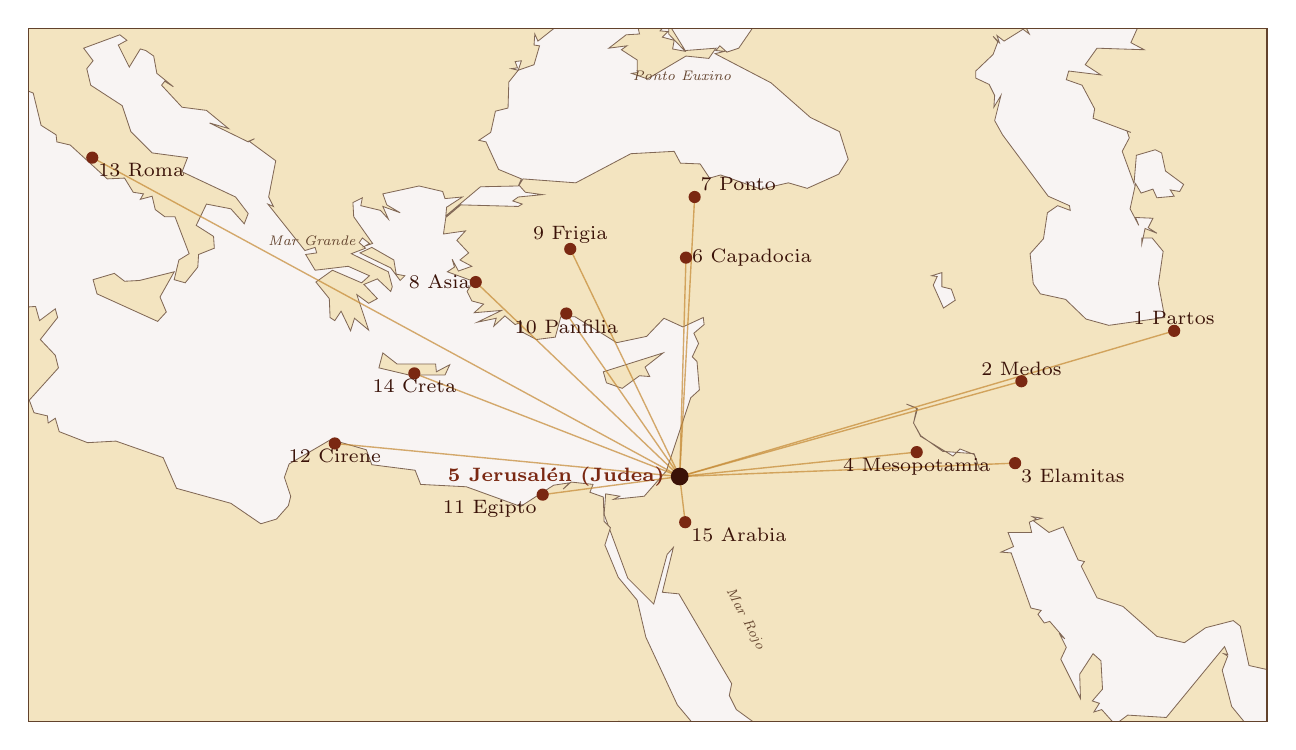
\begin{tikzpicture}[x=1cm,y=1cm,tierra/.style={fill=papiro,draw=sepia!80,line width=0.3pt},lago/.style={fill=tierraroja!5!white,draw=sepia!80,line width=0.3pt}]
\begin{scope}
\clip (0,0) rectangle (15.73,8.8);
\fill[tierraroja!5!white] (0,0) rectangle (15.73,8.8);
\fill[tierra] (16.71,0.44) -- (15.50,0.71) -- (15.39,1.21) -- (15.30,1.28) -- (14.95,1.19) -- (14.68,1.00) -- (14.33,1.08) -- (13.90,1.46) -- (13.57,1.57) -- (13.37,1.97) -- (13.41,2.03) -- (13.33,2.05) -- (13.14,2.47) -- (12.96,2.40) -- (12.76,2.55) -- (12.87,2.58) -- (12.75,2.60) -- (12.80,2.57) -- (12.71,2.53) -- (12.74,2.40) -- (12.44,2.40) -- (12.51,2.22) -- (12.35,2.15) -- (12.48,2.14) -- (12.73,1.44) -- (12.86,1.41) -- (12.82,1.36) -- (12.90,1.25) -- (12.97,1.27) -- (13.16,1.05) -- (13.10,1.10) -- (13.18,0.94) -- (13.11,0.79) -- (13.36,0.29) -- (13.35,0.60) -- (13.52,0.86) -- (13.62,0.77) -- (13.64,0.41) -- (13.51,0.26) -- (13.60,0.23) -- (13.53,0.12) -- (13.63,0.15) -- (13.80,-0.04) -- (13.96,0.08) -- (14.45,0.05) -- (15.19,0.95) -- (15.23,0.85) -- (15.18,0.86) -- (15.23,0.83) -- (15.16,0.65) -- (15.28,0.19) -- (15.46,-0.03) -- (15.97,-0.19) -- (16.22,-0.58) -- (16.32,-0.59) -- (16.17,-1.03) -- (15.90,-1.20) -- (15.80,-1.20) -- (15.65,-1.20) -- (9.99,-1.20) -- (9.74,-1.20) -- (9.57,-1.17) -- (9.48,-0.79) -- (9.55,-0.64) -- (9.32,-0.09) -- (8.99,0.15) -- (8.90,0.33) -- (8.93,0.48) -- (8.26,1.62) -- (8.05,1.64) -- (8.19,2.21) -- (8.11,2.12) -- (7.94,1.49) -- (7.61,1.82) -- (7.31,2.63) -- (7.33,2.89) -- (7.51,2.86) -- (7.43,2.82) -- (7.82,2.86) -- (8.10,3.18) -- (8.41,4.11) -- (8.52,4.21) -- (8.49,4.57) -- (8.43,4.63) -- (8.51,4.80) -- (8.45,4.93) -- (8.58,5.04) -- (8.57,5.13) -- (8.31,5.01) -- (8.07,5.12) -- (7.85,4.89) -- (7.47,4.81) -- (6.94,5.14) -- (6.76,5.14) -- (6.69,4.88) -- (6.45,4.85) -- (6.26,4.95) -- (6.26,5.07) -- (6.18,5.04) -- (6.05,5.15) -- (5.91,5.02) -- (5.94,5.12) -- (5.70,5.07) -- (6.01,5.22) -- (5.66,5.19) -- (5.78,5.30) -- (5.63,5.34) -- (5.57,5.46) -- (5.65,5.59) -- (5.32,5.71) -- (5.41,5.77) -- (5.38,5.87) -- (5.46,5.72) -- (5.63,5.78) -- (5.48,5.86) -- (5.59,5.95) -- (5.44,6.11) -- (5.55,6.23) -- (5.27,6.19) -- (5.30,6.40) -- (5.49,6.56) -- (6.22,6.54) -- (6.27,6.57) -- (6.15,6.61) -- (6.22,6.66) -- (6.53,6.69) -- (6.31,6.72) -- (6.23,6.81) -- (6.28,6.89) -- (6.95,6.84) -- (7.65,7.21) -- (8.20,7.24) -- (8.28,7.09) -- (8.53,7.08) -- (8.65,6.90) -- (8.79,6.94) -- (9.30,6.76) -- (9.65,6.84) -- (9.89,6.77) -- (10.29,6.95) -- (10.41,7.14) -- (10.30,7.49) -- (9.93,7.67) -- (9.43,8.11) -- (8.72,8.48) -- (8.84,8.51) -- (8.73,8.52) -- (8.78,8.58) -- (8.87,8.50) -- (9.02,8.55) -- (9.26,8.90) -- (9.37,8.81) -- (9.07,9.08) -- (9.37,9.06) -- (9.32,9.14) -- (9.60,9.21) -- (9.59,9.30) -- (9.03,9.24) -- (8.56,9.00) -- (8.61,9.05) -- (8.49,9.06) -- (8.19,8.83) -- (8.31,8.94) -- (8.25,9.01) -- (8.02,8.77) -- (8.12,8.76) -- (8.05,8.69) -- (8.20,8.65) -- (8.18,8.54) -- (8.34,8.51) -- (8.13,8.73) -- (8.13,8.86) -- (8.34,8.52) -- (8.73,8.55) -- (8.64,8.42) -- (8.35,8.45) -- (7.86,8.16) -- (7.66,8.23) -- (7.73,8.24) -- (7.73,8.40) -- (7.53,8.53) -- (7.60,8.58) -- (7.37,8.55) -- (7.59,8.72) -- (7.76,8.73) -- (7.73,8.86) -- (7.39,8.83) -- (7.14,8.91) -- (7.22,8.98) -- (7.05,9.03) -- (7.31,8.99) -- (7.20,9.16) -- (7.14,9.04) -- (7.02,9.05) -- (7.07,9.14) -- (7.02,9.05) -- (6.80,9.02) -- (6.71,8.83) -- (6.60,8.95) -- (6.71,8.83) -- (6.47,8.64) -- (6.43,8.73) -- (6.42,8.59) -- (6.49,8.58) -- (6.42,8.34) -- (6.22,8.27) -- (6.26,8.39) -- (6.18,8.38) -- (6.21,8.30) -- (6.13,8.29) -- (6.22,8.27) -- (6.10,8.12) -- (6.09,7.79) -- (5.93,7.75) -- (5.87,7.48) -- (5.72,7.38) -- (5.81,7.36) -- (5.97,7.01) -- (6.26,6.89) -- (6.22,6.80) -- (5.74,6.79) -- (5.30,6.42) -- (5.31,6.53) -- (5.51,6.66) -- (5.29,6.64) -- (5.26,6.73) -- (4.96,6.80) -- (4.50,6.70) -- (4.55,6.56) -- (4.72,6.46) -- (4.50,6.54) -- (4.57,6.38) -- (4.47,6.49) -- (4.22,6.55) -- (4.24,6.65) -- (4.12,6.59) -- (4.13,6.41) -- (4.37,6.07) -- (4.28,6.04) -- (4.33,6.07) -- (4.24,6.14) -- (4.20,6.08) -- (4.28,6.01) -- (4.10,5.94) -- (4.57,5.71) -- (4.62,5.52) -- (4.60,5.46) -- (4.43,5.62) -- (4.26,5.55) -- (4.43,5.37) -- (4.32,5.31) -- (4.17,5.42) -- (4.32,4.97) -- (4.14,5.12) -- (4.09,4.96) -- (3.97,5.21) -- (3.89,5.09) -- (3.83,5.13) -- (3.82,5.37) -- (3.65,5.58) -- (3.86,5.73) -- (4.23,5.57) -- (4.33,5.66) -- (4.06,5.78) -- (3.64,5.73) -- (3.52,5.93) -- (3.66,5.95) -- (3.64,6.02) -- (3.51,5.98) -- (3.04,6.57) -- (3.11,6.54) -- (3.05,6.66) -- (3.14,7.12) -- (2.80,7.37) -- (2.87,7.40) -- (2.79,7.36) -- (2.30,7.60) -- (2.54,7.53) -- (2.26,7.76) -- (1.95,7.80) -- (1.69,8.08) -- (1.73,8.13) -- (1.84,8.06) -- (1.63,8.23) -- (1.59,8.45) -- (1.49,8.52) -- (1.42,8.54) -- (1.28,8.31) -- (1.14,8.59) -- (1.25,8.65) -- (1.16,8.72) -- (0.70,8.55) -- (0.82,8.39) -- (0.74,8.29) -- (0.79,8.08) -- (1.19,7.82) -- (1.30,7.49) -- (1.57,7.22) -- (2.02,7.16) -- (1.95,6.98) -- (2.63,6.66) -- (2.79,6.45) -- (2.74,6.32) -- (2.57,6.51) -- (2.26,6.57) -- (2.13,6.30) -- (2.35,6.16) -- (2.36,6.01) -- (2.16,5.93) -- (2.15,5.77) -- (1.99,5.57) -- (1.85,5.61) -- (1.91,5.86) -- (2.04,5.94) -- (1.86,6.41) -- (1.73,6.41) -- (1.61,6.50) -- (1.57,6.67) -- (1.42,6.63) -- (1.46,6.70) -- (1.33,6.72) -- (1.22,6.90) -- (1.00,6.89) -- (0.53,7.32) -- (0.36,7.36) -- (0.35,7.45) -- (0.16,7.57) -- (0.06,7.98) -- (-0.41,8.17) -- (-0.63,7.96) -- (-0.92,7.88) -- (-0.98,7.67) -- (-0.98,7.64) -- (-0.98,10.00) -- (16.71,10.00) -- (16.71,0.44) -- cycle;
\fill[tierra] (7.30,2.85) -- (7.31,2.54) -- (7.39,2.46) -- (7.32,2.24) -- (7.49,1.83) -- (7.73,1.54) -- (7.84,1.07) -- (8.24,0.21) -- (8.45,-0.04) -- (8.35,-0.03) -- (8.41,-0.42) -- (8.81,-0.77) -- (8.84,-1.04) -- (8.95,-1.17) -- (8.88,-1.11) -- (8.91,-1.20) -- (-0.98,-1.20) -- (-0.98,5.15) -- (-0.98,5.21) -- (-0.98,5.15) -- (-0.86,5.23) -- (-0.69,5.14) -- (-0.08,5.34) -- (-0.06,5.26) -- (0.09,5.27) -- (0.14,5.09) -- (0.34,5.24) -- (0.37,5.13) -- (0.15,4.85) -- (0.34,4.65) -- (0.38,4.49) -- (0.01,4.08) -- (0.07,3.92) -- (0.24,3.88) -- (0.25,3.79) -- (0.34,3.85) -- (0.39,3.68) -- (0.75,3.54) -- (1.11,3.56) -- (1.71,3.35) -- (1.88,2.96) -- (2.57,2.77) -- (2.95,2.51) -- (3.15,2.57) -- (3.30,2.74) -- (3.33,2.86) -- (3.25,3.10) -- (3.31,3.27) -- (3.84,3.58) -- (4.29,3.45) -- (4.36,3.26) -- (4.91,3.19) -- (4.98,3.01) -- (5.56,2.98) -- (6.25,2.73) -- (6.67,3.00) -- (6.87,3.03) -- (6.79,2.95) -- (6.89,3.04) -- (7.17,3.01) -- (7.13,2.91) -- (7.30,2.85) -- cycle;
\fill[tierra] (1.64,5.08) -- (0.87,5.43) -- (0.82,5.61) -- (1.09,5.69) -- (1.22,5.59) -- (1.41,5.60) -- (1.85,5.71) -- (1.67,5.39) -- (1.75,5.20) -- (1.64,5.08) -- cycle;
\fill[tierra] (-0.51,6.00) -- (-0.47,6.33) -- (-0.60,6.78) -- (-0.47,6.73) -- (-0.25,6.90) -- (-0.16,6.86) -- (-0.06,6.61) -- (-0.12,6.50) -- (-0.12,6.12) -- (-0.16,6.04) -- (-0.32,6.11) -- (-0.37,5.95) -- (-0.51,6.00) -- cycle;
\fill[tierra] (7.54,4.23) -- (7.34,4.30) -- (7.30,4.44) -- (8.06,4.68) -- (7.83,4.50) -- (7.89,4.38) -- (7.76,4.39) -- (7.54,4.23) -- cycle;
\fill[tierra] (-0.33,6.99) -- (-0.44,7.10) -- (-0.39,7.16) -- (-0.46,7.16) -- (-0.41,7.22) -- (-0.48,7.35) -- (-0.23,7.47) -- (-0.19,7.61) -- (-0.15,7.25) -- (-0.26,6.95) -- (-0.33,6.99) -- cycle;
\fill[tierra] (4.83,4.40) -- (4.45,4.49) -- (4.50,4.68) -- (4.68,4.54) -- (5.17,4.54) -- (5.18,4.44) -- (5.35,4.53) -- (5.29,4.40) -- (4.83,4.40) -- cycle;
\fill[tierra] (4.72,5.60) -- (4.60,5.76) -- (4.21,5.95) -- (4.36,6.02) -- (4.64,5.86) -- (4.67,5.68) -- (4.78,5.66) -- (4.72,5.60) -- cycle;
\fill[lago] (12.89,6.13) -- (12.94,6.46) -- (13.07,6.55) -- (13.23,6.49) -- (13.22,6.55) -- (12.95,6.67) -- (12.37,7.45) -- (12.27,7.63) -- (12.35,7.95) -- (12.26,7.80) -- (12.27,7.95) -- (12.20,8.09) -- (12.03,8.17) -- (12.03,8.26) -- (12.25,8.47) -- (12.31,8.63) -- (12.25,8.70) -- (12.33,8.62) -- (12.30,8.71) -- (12.39,8.64) -- (12.63,8.79) -- (12.71,8.73) -- (12.66,8.83) -- (12.88,8.90) -- (12.88,9.03) -- (13.04,9.01) -- (13.50,9.25) -- (13.83,9.12) -- (13.91,9.20) -- (14.11,9.16) -- (14.14,8.93) -- (14.00,8.62) -- (14.17,8.53) -- (13.57,8.55) -- (13.42,8.34) -- (13.62,8.21) -- (13.21,8.26) -- (13.18,8.15) -- (13.38,8.08) -- (13.54,7.78) -- (13.52,7.66) -- (14.00,7.48) -- (13.95,7.50) -- (13.98,7.41) -- (13.89,7.24) -- (14.04,6.83) -- (14.07,7.19) -- (14.31,7.26) -- (14.39,7.22) -- (14.44,6.99) -- (14.67,6.82) -- (14.62,6.73) -- (14.50,6.75) -- (14.55,6.67) -- (14.33,6.65) -- (14.28,6.76) -- (14.13,6.71) -- (14.06,6.83) -- (13.99,6.51) -- (14.10,6.30) -- (14.06,6.40) -- (14.28,6.39) -- (14.22,6.27) -- (14.33,6.20) -- (14.18,6.26) -- (14.14,6.07) -- (14.14,6.14) -- (14.27,6.14) -- (14.41,5.97) -- (14.35,5.56) -- (14.43,5.13) -- (13.72,5.03) -- (13.43,5.11) -- (13.17,5.36) -- (12.85,5.43) -- (12.76,5.56) -- (12.72,5.94) -- (12.89,6.13) -- cycle;
\fill[lago] (16.71,8.29) -- (16.71,8.26) -- (16.71,8.04) -- (16.70,8.13) -- (16.62,8.01) -- (16.71,7.85) -- (16.30,7.76) -- (16.32,7.86) -- (15.98,7.98) -- (16.05,7.87) -- (15.87,7.85) -- (15.79,8.34) -- (15.95,8.73) -- (16.18,8.82) -- (16.15,8.70) -- (16.22,8.73) -- (16.20,8.92) -- (16.30,8.94) -- (16.35,8.84) -- (16.42,8.91) -- (16.31,9.01) -- (16.49,9.09) -- (16.58,9.03) -- (16.54,9.12) -- (16.67,9.11) -- (16.65,9.03) -- (16.71,8.99) -- (16.71,9.15) -- (16.71,9.10) -- (16.71,8.86) -- (16.68,8.84) -- (16.71,8.76) -- (16.69,8.66) -- (16.71,8.71) -- (16.71,8.46) -- (16.71,8.42) -- (16.71,8.29) -- cycle;
\fill[lago] (7.16,10.00) -- (7.43,10.00) -- (7.61,10.00) -- (7.90,9.97) -- (8.11,9.80) -- (8.28,9.85) -- (8.21,9.64) -- (8.29,9.37) -- (7.88,9.36) -- (7.93,9.32) -- (7.77,9.14) -- (7.42,9.06) -- (7.72,9.14) -- (7.84,9.42) -- (8.19,9.42) -- (8.24,9.70) -- (8.21,9.78) -- (7.66,10.00) -- (7.53,9.99) -- (7.16,10.00) -- cycle;
\fill[lago] (11.60,5.70) -- (11.60,5.52) -- (11.72,5.49) -- (11.77,5.35) -- (11.62,5.25) -- (11.49,5.54) -- (11.54,5.65) -- (11.47,5.66) -- (11.60,5.70) -- cycle;
\fill[lago] (7.50,-0.01) -- (7.55,-0.19) -- (7.49,-0.35) -- (7.56,-0.44) -- (7.45,-0.38) -- (7.32,-0.59) -- (7.22,-0.53) -- (6.89,-1.00) -- (7.15,-0.61) -- (7.10,-0.54) -- (7.39,-0.49) -- (7.51,-0.28) -- (7.49,-0.19) -- (7.41,-0.20) -- (7.48,-0.18) -- (7.50,-0.01) -- cycle;
\fill[lago] (11.06,10.00) -- (11.15,10.00) -- (10.97,9.90) -- (11.07,9.87) -- (10.86,9.71) -- (10.84,9.48) -- (10.81,9.54) -- (10.54,9.41) -- (10.61,9.57) -- (10.55,9.60) -- (10.74,9.55) -- (10.73,9.66) -- (10.84,9.73) -- (10.79,9.82) -- (10.93,9.78) -- (10.96,9.91) -- (11.11,9.99) -- (11.14,10.00) -- (11.04,10.00) -- (11.00,10.00) -- (11.06,10.00) -- cycle;
\fill[lago] (11.33,9.81) -- (11.28,9.84) -- (11.45,10.00) -- (11.61,10.00) -- (11.33,9.81) -- cycle;
\fill[lago] (11.15,4.03) -- (11.29,3.97) -- (11.24,3.79) -- (11.33,3.63) -- (11.61,3.43) -- (12.01,3.40) -- (12.08,3.20) -- (12.01,3.39) -- (11.83,3.46) -- (11.74,3.37) -- (11.33,3.62) -- (11.24,3.79) -- (11.28,3.98) -- (11.15,4.03) -- cycle;
\end{scope}
\draw[sepia,line width=0.6pt] (0,0) rectangle (15.73,8.8);
\coordinate (J) at (8.27,3.11);
\foreach \p in {(14.55,4.96),(12.61,4.32),(12.53,3.28),(11.28,3.42),(8.35,5.89),(8.46,6.66),(5.68,5.58),(6.88,6.00),(6.83,5.18),(6.53,2.88),(3.89,3.53),(0.81,7.16),(4.90,4.42),(8.34,2.53)}
  \draw[mostaza!80!tierraroja,line width=0.5pt,opacity=0.7] (J) -- \p;
\foreach \p/\n/\pos in {(14.55,4.96)/{1 Partos}/above,(12.61,4.32)/{2 Medos}/above,(12.53,3.28)/{3 Elamitas}/below right,(11.28,3.42)/{4 Mesopotamia}/below,(8.35,5.89)/{6 Capadocia}/right,(8.46,6.66)/{7 Ponto}/above right,(5.68,5.58)/{8 Asia}/left,(6.88,6.00)/{9 Frigia}/above,(6.83,5.18)/{10 Panfilia}/below,(6.53,2.88)/{11 Egipto}/below left,(3.89,3.53)/{12 Cirene}/below,(0.81,7.16)/{13 Roma}/below right,(4.90,4.42)/{14 Creta}/below,(8.34,2.53)/{15 Arabia}/below right}{
  \fill[tierraroja] \p circle (2.2pt);
  \node[\pos,font=\scriptsize,text=caferojizo,inner sep=2pt] at \p {\n};}
\fill[caferojizo] (J) circle (3.2pt); \node[left=2pt,font=\scriptsize\bfseries,text=tierraroja] at (J) {5 Jerusalén (Judea)};
\node[font=\tiny\itshape,text=sepia] at (3.6,6.1) {Mar Grande};
\node[font=\tiny\itshape,text=sepia] at (8.3,8.2) {Ponto Euxino};
\node[font=\tiny\itshape,text=sepia,rotate=-62] at (9.1,1.3) {Mar Rojo};
\end{tikzpicture}\par
{\footnotesize\color{sepia}\textit{Figura 4.} Las naciones de Hch 2:9--11 y Jerusalén. \textit{Nota.} Elaboración propia; costas simplificadas (GSHHS, resolución baja) y ubicaciones aproximadas por coordenadas reales: Partia (Hecatómpilos), Media (Ecbatana), Elam (Susa), Mesopotamia (Babilonia), Capadocia (Cesarea Mazaca), Ponto (Amasía), Asia (Éfeso), Panfilia (Perge), Egipto (Alejandría), Creta (Gortina), Arabia (Petra).}
\end{center}

Algunos intérpretes leen la lista sobre el fondo de la Tabla de las Naciones de Génesis 10, con Jerusalén en el centro (Scott, 1994); otros la consideran un inventario de la diáspora judía conocida por Lucas (Fitzmyer, 1998). En ambos casos la escena dice lo mismo: el pueblo disperso entre las naciones se encuentra reunido en Jerusalén el día de la fiesta, y todos oyen ``en nuestras lenguas'' (\grc{ταῖς ἡμετέραις γλώσσαις}) un mismo mensaje.

\begin{center}
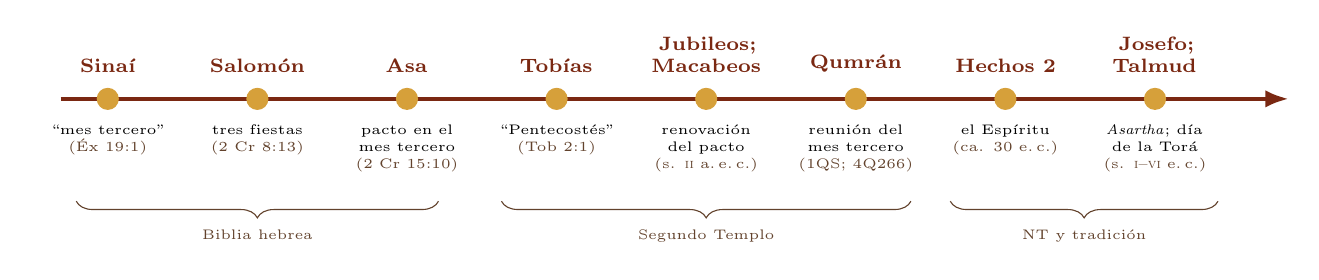
\begin{tikzpicture}[font=\scriptsize]
 \draw[line width=1.6pt,tierraroja,-{Latex[length=3mm]}] (0,0) -- (15.6,0);
 \foreach \x/\a/\b/\c in {0.6/{Sinaí}/{``mes tercero''}/{Éx 19:1},2.5/{Salomón}/{tres fiestas}/{2 Cr 8:13},4.4/{Asa}/{pacto en el mes tercero}/{2 Cr 15:10},6.3/{Tobías}/{``Pentecostés''}/{Tob 2:1},8.2/{Jubileos; Macabeos}/{renovación del pacto}/{s. \textsc{ii} a.\,e.\,c.},10.1/{Qumrán}/{reunión del mes tercero}/{1QS; 4Q266},12.0/{Hechos 2}/{el Espíritu}/{ca. 30 e.\,c.},13.9/{Josefo; Talmud}/{\emph{Asartha}; día de la Torá}/{s. \textsc{i}--\textsc{vi} e.\,c.}}{
   \fill[mostaza] (\x,0) circle (4pt);
   \node[above=6pt,font=\scriptsize\bfseries,text=tierraroja,text width=1.8cm,align=center] at (\x,0) {\a};
   \node[below=6pt,text width=1.8cm,align=center,font=\tiny] at (\x,0) {\b\\ \textcolor{sepia}{(\c)}};}
 \draw[decorate,decoration={brace,amplitude=6pt,mirror},sepia] (0.2,-1.3) -- (4.8,-1.3) node[midway,below=7pt,font=\tiny,text=sepia] {Biblia hebrea};
 \draw[decorate,decoration={brace,amplitude=6pt,mirror},sepia] (5.6,-1.3) -- (10.8,-1.3) node[midway,below=7pt,font=\tiny,text=sepia] {Segundo Templo};
 \draw[decorate,decoration={brace,amplitude=6pt,mirror},sepia] (11.3,-1.3) -- (14.7,-1.3) node[midway,below=7pt,font=\tiny,text=sepia] {NT y tradición};
\end{tikzpicture}\par
{\footnotesize\color{sepia}\textit{Figura 5.} Shavuot en la historia: del mes tercero del Sinaí a la tradición rabínica. \textit{Nota.} Elaboración propia; las fechas de Jubileos, Qumrán y el Talmud son aproximadas.}
\end{center}

%===================================================================
\section{Lectura filológica}

\subsection{El nombre: semanas, siete y juramento}

\begin{filologia}[\emph{shavuot}, \emph{sheva}, \emph{shevuá}]
\begin{tabular}{@{}L{3.3cm}L{1.5cm}L{9.85cm}@{}}
\heb{שֶׁבַע} \emph{sheva} & \heb{שׁבע} & ``siete''. La raíz da el número y sus derivados: \heb{שְׁבִיעִי} (\emph{shevi'í}), ``séptimo''; \heb{שִׁבְעָה} (\emph{shiv'á}) ``siete'' con sustantivo masculino (Dt 16:9). \\[2pt]
\heb{שָׁבוּעַ} \emph{shavúa} & \heb{שׁבע} & ``semana'', una unidad de siete (días o años: Dn 9:24--27). Plural \heb{שָׁבֻעוֹת} (\emph{shavuot}): ``semanas''. \\[2pt]
\heb{חַג שָׁבֻעֹת} \emph{jag shavuot} & \heb{חגג} & ``fiesta de las semanas'' (Éx 34:22; Dt 16:10, 16). \emph{Jag} es la fiesta de peregrinación, de la raíz ``hacer ronda, peregrinar''; cf. árabe \emph{hajj}. \\[2pt]
\heb{שְׁבוּעָה} \emph{shevuá} & \heb{שׁבע} & ``juramento'' (nifal \heb{נִשְׁבַּע}, ``jurar''): quizá ``atarse por siete'' (cf. las siete corderas de Gn 21:28--31, Beerseba). En texto consonántico, el plural ``juramentos'' y ``semanas'' se escriben igual: \heb{שבעות}. \\[2pt]
\heb{שַׁבָּתוֹת תְּמִימֹת} & \heb{שׁבת} & En Lv 23:15 las semanas se llaman \emph{shabatot}, ``sábados''; la palabra \emph{shavuot} no aparece en Levítico. \\
\end{tabular}
\end{filologia}

La homografía de \heb{שבעות} permitió a la predicación judía posterior un juego de palabras: Shavuot como fiesta de las ``semanas'' y de los ``juramentos'', el de Dios a los padres y el de Israel en el Sinaí. El juego es homilético, porque la vocalización los distingue (\emph{shavuot} / \emph{shevu'ot}); su base bíblica más cercana es 2~Cr 15:14--15, donde el pacto del mes tercero se sella con ``juramento''. Jeremías, por su parte, muestra la palabra ``semanas'' dentro del lenguaje de la siega: el \SENOR{} ``da lluvia temprana y tardía en su tiempo, y nos guarda los tiempos establecidos de la siega'' (Jer 5:24). Lo que la RVR1960 traduce ``tiempos establecidos'' es \heb{שְׁבֻעֹת חֻקּוֹת קָצִיר} (\emph{shevu'ot juqot qatsir}), literalmente ``las semanas fijadas de la siega'', y así un solo versículo reúne las dos lluvias y las semanas de Shavuot.

\subsection{La cuenta: cumplidas y cincuenta}

\begin{filologia}[\emph{temimot} y \emph{jamishim yom}]
\begin{tabular}{@{}L{3.3cm}L{1.5cm}L{9.85cm}@{}}
\heb{וּסְפַרְתֶּם} \emph{usfartem} & \heb{ספר} & ``y contaréis''. El verbo de contar es el de ``escribir'' y ``relatar'' (\emph{séfer}, libro; \emph{sofer}, escriba). La misma forma abre la cuenta del Jubileo (\heb{וְסָפַרְתָּ}, Lv 25:8). \\[2pt]
\heb{תְּמִימֹת} \emph{temimot} & \heb{תמם} & ``completas, cumplidas'', femenino plural de \emph{tamim}, el adjetivo de la víctima ``sin defecto'' (Lv 23:12, 18) y del hombre ``perfecto'' (Gn 6:9; 17:1). Las semanas deben estar enteras, sin faltar días. \\[2pt]
\heb{חֲמִשִּׁים יוֹם} \emph{jamishim yom} & \heb{חמשׁ} & ``cincuenta días''. El hebreo usa el singular \emph{yom} tras decenas. La LXX traduce \grc{πεντήκοντα ἡμέρας}. \\[2pt]
\heb{מִנְחָה חֲדָשָׁה} \emph{minjá jadashá} & \heb{חדשׁ} & ``ofrenda nueva'' (Lv 23:16; Nm 28:26), hecha con el grano del año. Es el adjetivo de ``pacto nuevo'' (\heb{בְּרִית חֲדָשָׁה}, Jer 31:31) y ``corazón nuevo'' (Ez 36:26). \\
\end{tabular}
\end{filologia}

\subsection{La siega y sus primicias}

\begin{filologia}[\emph{qatsir} y \emph{bikurim}]
\begin{tabular}{@{}L{3.3cm}L{1.5cm}L{9.85cm}@{}}
\heb{קָצִיר} \emph{qatsir} & \heb{קצר} & ``siega'' del grano, el acto y su tiempo. \heb{חַג הַקָּצִיר}, ``fiesta de la siega'' (Éx 23:16). Se distingue de \heb{אָסִיף} (\emph{asif}), la ``cosecha'' o acopio de otoño (Sukkot, Éx 23:16b). \\[2pt]
\heb{חֶרְמֵשׁ} \emph{jármesh} & --- & ``hoz'' (Dt 16:9; 23:25). La cuenta de Deuteronomio comienza con la primera hoz en el grano en pie (\heb{קָמָה}, \emph{qamá}). \\[2pt]
\heb{בִּכּוּרִים} \emph{bikurim} & \heb{בכר} & ``primicias'', lo primero que madura; la raíz de \heb{בְּכוֹר} (\emph{bejor}), ``primogénito''. \heb{יוֹם הַבִּכּוּרִים}, ``día de las primicias'' (Nm 28:26). \\[2pt]
\heb{חִטִּים} \emph{jitim} & \heb{חטה} & ``trigo'' (plural de \emph{jitá}): \emph{bikuré qetsir jitim}, ``primicias de la siega del trigo'' (Éx 34:22); frente a \heb{שְׂעֹרִים} (\emph{se'orim}), ``cebada'' (Rt 1:22). \\[2pt]
\grc{ἀπαρχή} \emph{aparchē} & --- & ``primicia'' en la LXX y en Pablo: Cristo ``primicias de los que durmieron'' (1~Co 15:20); ``las primicias del Espíritu'' (Ro 8:23). \\
\end{tabular}
\end{filologia}

\subsection{Leudado y mecido}

\begin{filologia}[\emph{jamets} y \emph{tenufá}]
\begin{tabular}{@{}L{3.3cm}L{1.5cm}L{9.85cm}@{}}
\heb{חָמֵץ} \emph{jamets} & \heb{חמץ} & ``lo leudado'', ``fermentado''. Prohibido en Pésaj y Matsot (Éx 12:15) y en el altar: ``ninguna ofrenda que ofreciereis a \SENOR{} será con levadura'' (Lv 2:11). Excepción expresa: las primicias leudadas pueden ofrecerse, ``mas no subirán sobre el altar en olor grato'' (Lv 2:12); también el pan de la acción de gracias (Lv 7:13). \\[2pt]
\heb{שְׂאֹר} \emph{se'or} & --- & ``levadura'' como masa madre (Éx 12:15; Lv 2:11), distinta del producto leudado (\emph{jamets}). \\[2pt]
\heb{תְּנוּפָה} \emph{tenufá} & \heb{נוף} & ``ofrenda mecida'', de \emph{henif}, ``mover de un lado a otro, alzar''. Se aplica al \emph{ómer} (Lv 23:15), a los dos panes (\heb{לֶחֶם תְּנוּפָה}, v. 17) y a los corderos de paz (v. 20). Milgrom (1991) sostiene que el gesto es una elevación ante el santuario más que un balanceo. \\[2pt]
\heb{סֹלֶת} \emph{sólet} & --- & ``flor de harina'', sémola fina; \heb{שְׁנֵי עֶשְׂרֹנִים} (\emph{shené esronim}), ``dos décimas'' de efa (cerca de cuatro litros en total; las equivalencias son aproximadas). \\
\end{tabular}
\end{filologia}

El detalle de Lv 2:12 importa para la lectura de los dos panes. La misma ley que prohíbe la levadura en el altar prevé la excepción de las primicias, con una condición: no se queman. Los panes de Shavuot se mecen ante el \SENOR{} y quedan para el sacerdote (Lv 23:20), sin tocar el fuego del altar. El documento de referencia de la serie cita Lv 2:4--5 (las tortas cocidas al horno, ``sin levadura'') como prueba de la prohibición; el texto que la formula en general es Lv 2:11, y el que prevé la excepción, Lv 2:12.

\subsection{Rincón y espiga}

\begin{filologia}[\emph{peá} y \emph{léqet}]
\begin{tabular}{@{}L{3.3cm}L{1.5cm}L{9.85cm}@{}}
\heb{פְּאַת שָׂדְךָ} \emph{pe'at sadjá} & \heb{פאה} & ``el rincón de tu campo''. \emph{Peá} es borde, extremo: la misma palabra designa el borde de la barba y de la cabeza (Lv 19:27). La ley no fija la medida; la Misná dedica un tratado entero a ella (\emph{Peá}) y fija un mínimo de una sexagésima parte (m. Peá 1:2), como tradición posterior. \\[2pt]
\heb{לֶקֶט קְצִירְךָ} \emph{léqet qetsirjá} & \heb{לקט} & ``el espigueo de tu siega'': las espigas que caen al segar. El verbo \emph{laqat} es el que define a Rut (Rt 2:2, 3, 7, 8). \\[2pt]
\heb{לֶעָנִי וְלַגֵּר} & \heb{ענה}; \heb{גור} & ``para el pobre y para el extranjero''. \emph{Guer} es el residente sin tierra; Dt 16:11 añade al huérfano y a la viuda. \\[2pt]
\heb{תַּעֲזֹב} \emph{ta'azov} & \heb{עזב} & ``dejarás'', ``abandonarás'': el dueño debe soltar lo que podría recoger. \\
\end{tabular}
\end{filologia}

\subsection{El lenguaje del Sinaí}

\needspace{5\baselineskip}\hebverso{וְכָל־הָעָם רֹאִים אֶת־הַקּוֹלֹת וְאֶת־הַלַּפִּידִם וְאֵת קוֹל הַשֹּׁפָר וְאֶת־הָהָר עָשֵׁן}
\begin{cita}Todo el pueblo observaba el estruendo y los relámpagos, y el sonido de la bocina, y el monte que humeaba; y viéndolo el pueblo, temblaron, y se pusieron de lejos.\fuente{(Éx 20:18)}\end{cita}

\begin{filologia}[\emph{qolot}, \emph{esh}, \emph{lapid}]
\begin{tabular}{@{}L{3.3cm}L{1.5cm}L{9.85cm}@{}}
\heb{קֹלֹת} \emph{qolot} & \heb{קול} & ``voces''. En plural designa los truenos (Éx 9:23; 19:16; 1~S 12:17); en singular, \heb{קוֹל} es ``voz'', ``sonido'': \heb{קֹל שֹׁפָר}, ``sonido de bocina'' (Éx 19:16). La RVR1960 traduce ``truenos'' (19:16) y ``estruendo'' (20:18). \\[2pt]
\heb{רֹאִים אֶת־הַקּוֹלֹת} & \heb{ראה} & ``veían las voces'' (Éx 20:18). El hebreo une vista y oído; la RVR1960 suaviza con ``observaba''. \\[2pt]
\heb{אֵשׁ} \emph{esh} & --- & ``fuego'': ``\SENOR{} había descendido sobre él en fuego'' (Éx 19:18); ``habló\ldots{} de en medio del fuego'' (Dt 4:12; 5:22). \\[2pt]
\heb{לַפִּידִם} \emph{lapidim} & --- & ``antorchas'', ``llamas'' (RVR1960: ``relámpagos''). La misma palabra designa la ``antorcha de fuego'' que pasó entre los animales partidos en el pacto con Abram (\heb{לַפִּיד אֵשׁ}, Gn 15:17). \\[2pt]
\heb{קוֹל גָּדוֹל} \emph{qol gadol} & --- & ``gran voz'' (Dt 5:22), ``y no añadió más'': la voz del Decálogo es única. \\
\end{tabular}
\end{filologia}

Filón de Alejandría, contemporáneo de los apóstoles, comentó la escena del Sinaí con una imagen que se acerca mucho a Hechos 2. Según él, Dios no habló con boca; formó en el aire un sonido invisible que se convirtió en ``fuego en forma de llama'' (\emph{De Decalogo} 33), y de en medio del fuego que bajaba del cielo resonó una voz, mientras la llama se articulaba en el lenguaje familiar de los oyentes (\grc{τῆς φλογὸς εἰς διάλεκτον ἀρθρουμένης τὴν συνήθη τοῖς ἀκροωμένοις}, \emph{De Decalogo} 46). Filón no menciona Shavuot en ese pasaje ni habla de varias lenguas; habla de una voz de fuego que se vuelve lenguaje humano, lo cual basta para mostrar que la exégesis judía del siglo \textsc{i} ya leía el Sinaí como fuego que habla.

\subsection{El lenguaje de Hechos 2}

\begin{filologia}[Hch 2:1--6]
\begin{tabular}{@{}L{3.5cm}L{1.3cm}L{9.85cm}@{}}
\grc{ἐν τῷ συμπληροῦσθαι} & \grc{πληρόω} & ``al cumplirse'' (v. 1); RVR1960: ``cuando llegó''. El compuesto con \grc{σύν} subraya que el plazo se completa: la cuenta de cincuenta días llega a su término. Lucas usa la misma forma en Lc 9:51 (``cuando se cumplió el tiempo''). \\[2pt]
\grc{ἦχος} \emph{ēchos} & --- & ``estruendo'', sonido fuerte (v. 2). Hebreos usa la palabra para el Sinaí: \grc{σάλπιγγος ἤχῳ καὶ φωνῇ ῥημάτων}, ``el sonido de la trompeta y la voz que hablaba'' (He 12:19). \\[2pt]
\grc{πνοῆς βιαίας} \emph{pnoēs biaias} & \grc{πνέω} & ``viento recio'' (v. 2), literalmente ``soplo violento''. \emph{Pnoē} pertenece a la familia de \grc{πνεῦμα} (Espíritu, viento); el hebreo \heb{רוּחַ} (\emph{rúaj}) cubre ambos sentidos (Ez 37:9--14; Jn 3:8). \\[2pt]
\grc{γλῶσσαι ὡσεὶ πυρός} & --- & ``lenguas como de fuego'' (v. 3). \emph{Glōssa} es el órgano y el idioma; \grc{ὡσεί} marca comparación: Lucas describe lo que se vio, no la sustancia. \\[2pt]
\grc{ἑτέραις γλώσσαις} & --- & ``en otras lenguas'' (v. 4), entendidas por cada oyente ``en su propia lengua'' (\grc{τῇ ἰδίᾳ διαλέκτῳ}, v. 6). \\[2pt]
\grc{φωνῆς} \emph{phōnēs} & --- & ``este estruendo'' (v. 6), literalmente ``esta voz'': el término griego que traduce \emph{qol}. \\
\end{tabular}
\end{filologia}

\subsection{Pentecostés: del hebreo al español}

El nombre griego traduce ``cincuenta'', y ya no ``semanas''. La Septuaginta del Pentateuco conserva el nombre hebreo traducido (\grc{ἑορτὴ ἑβδομάδων}, ``fiesta de semanas'', Éx 34:22; Dt 16:10); los escritos judíos en griego de los siglos \textsc{ii}--\textsc{i} a.\,e.\,c. adoptan el ordinal \grc{πεντηκοστή}, ``la quincuagésima'' (sobrentendido \grc{ἡμέρα}, ``día''). El Nuevo Testamento hereda ese uso, y el latín lo transcribe como \emph{Pentecoste}.

\begin{center}
\begin{tikzpicture}[font=\small,node distance=0.55cm,
  bx/.style={draw=tierraroja,line width=0.8pt,fill=papiro,rounded corners=3pt,text width=3.0cm,align=center,inner sep=5pt,minimum height=2.5cm}]
 \node[bx] (h) {\textbf{Hebreo}\\ \heb{חַג שָׁבֻעוֹת}\\ \emph{jag shavuot}\\ {\footnotesize ``fiesta de las semanas''}\\ {\scriptsize\color{sepia}Éx 34:22; Dt 16:10}};
 \node[bx,right=of h] (l) {\textbf{LXX Pentateuco}\\ \grc{ἑορτὴ ἑβδομάδων}\\ {\footnotesize ``fiesta de semanas''}\\ {\scriptsize\color{sepia}Éx 34:22; Dt 16:10}};
 \node[bx,right=of l] (g) {\textbf{Griego judío}\\ \grc{πεντηκοστή}\\ {\footnotesize ``el quincuagésimo [día]''}\\ {\scriptsize\color{sepia}Tob 2:1; 2 Mac 12:32; Josefo}};
 \node[bx,right=of g,draw=mostaza,line width=1.4pt,fill=tierraroja,text=papiro] (n) {\textbf{NT}\\ \grc{ἡ ἡμέρα τῆς πεντηκοστῆς}\\ {\footnotesize ``el día de Pentecostés''}\\ {\scriptsize Hch 2:1; 20:16; 1 Co 16:8}};
 \draw[-{Latex[length=3mm]},mostaza!80!tierraroja,line width=1.3pt] (h)--(l);
 \draw[-{Latex[length=3mm]},mostaza!80!tierraroja,line width=1.3pt] (l)--(g);
 \draw[-{Latex[length=3mm]},mostaza!80!tierraroja,line width=1.3pt] (g)--(n);
 \node[below=0.35cm of l.south east,anchor=north,font=\footnotesize\itshape,text=sepia,text width=13cm,align=center] {el nombre pasa de la unidad contada (semanas) al día al que se llega (cincuenta) $\rightarrow$ latín \emph{Pentecoste} $\rightarrow$ español \emph{Pentecostés}; arameo \emph{Asartha} y hebreo rabínico \emph{Atséret}, ``asamblea de clausura''};
\end{tikzpicture}\par
{\footnotesize\color{sepia}\textit{Figura 6.} Del hebreo \emph{shavuot} al español \emph{Pentecostés}. \textit{Nota.} Elaboración propia con la BHS, la LXX (Rahlfs-Hanhart), NA28 y Josefo, \emph{Ant.} 3.252.}
\end{center}

\subsection{Las lluvias: \emph{yoré}, \emph{malqosh} y el \emph{moré} de Joel 2:23}

Las dos lluvias del año agrícola tienen nombre propio, y aparecen juntas como bendición del pacto:

\begin{cita}Yo daré la lluvia de vuestra tierra a su tiempo, la temprana y la tardía; y recogerás tu grano, tu vino y tu aceite.\fuente{(Dt 11:14)}\end{cita}

\needspace{5\baselineskip}\hebverso{וּבְנֵי צִיּוֹן גִּילוּ וְשִׂמְחוּ בַּיהוָה אֱלֹהֵיכֶם כִּי־נָתַן לָכֶם אֶת־הַמּוֹרֶה לִצְדָקָה \\ וַיּוֹרֶד לָכֶם גֶּשֶׁם מוֹרֶה וּמַלְקוֹשׁ בָּרִאשׁוֹן}
\begin{cita}Vosotros también, hijos de Sion, alegraos y gozaos en \SENOR{} vuestro Dios; porque os ha dado la primera lluvia a su tiempo, y hará descender sobre vosotros lluvia temprana y tardía como al principio.\fuente{(Jl 2:23)}\end{cita}

\begin{filologia}[Jl 2:23 y las lluvias]
\begin{tabular}{@{}L{3.3cm}L{1.5cm}L{9.85cm}@{}}
\heb{יוֹרֶה} / \heb{מוֹרֶה} \emph{yoré} / \emph{moré} & \heb{ירה} & ``lluvia temprana'' de otoño (Dt 11:14; Jer 5:24). \emph{Moré} (Jl 2:23b; Sal 84:6 [84:7]) es variante de \emph{yoré}. La raíz \emph{yarah} significa ``lanzar'' (flechas, agua) y, en hifil, ``enseñar'': de ahí \heb{תּוֹרָה} (\emph{torá}) y \heb{מוֹרֶה} (\emph{moré}), ``maestro'' (Is 30:20). \\[2pt]
\heb{מַלְקוֹשׁ} \emph{malqosh} & \heb{לקשׁ} & ``lluvia tardía'' de primavera, la que llena la espiga antes de la siega (Dt 11:14; Jer 5:24; Os 6:3; Za 10:1; Pr 16:15). \\[2pt]
\heb{גֶּשֶׁם} \emph{guéshem} & --- & ``lluvia'' en general, la de invierno (Jl 2:23; Lv 26:4). \\[2pt]
\heb{הַמּוֹרֶה לִצְדָקָה} & \heb{צדק} & ``el \emph{moré} para justicia'' (v. 23a). Con artículo y seguido de \emph{litsdaká}: puede ser ``la lluvia temprana en su justa medida'' (RVR1960 ``a su tiempo''; RV 1909 ``arregladamente'') o ``el maestro de justicia'' (Vulgata \emph{doctorem iustitiae}). Ver recuadro. \\[2pt]
\heb{בָּרִאשׁוֹן} \emph{barishón} & \heb{ראשׁ} & ``en el primero'', ``como al principio''. La LXX lee \grc{καθὼς ἔμπροσθεν}, ``como antes''; muchos modernos entienden ``en el [mes] primero'' (Nisán). \\[2pt]
\grc{πρόϊμος καὶ ὄψιμος} & --- & ``temprana y tardía'' en la LXX (Dt 11:14; Jl 2:23) y en Stg 5:7. \\
\end{tabular}
\end{filologia}

\begin{nota}[Precisión: \emph{moré litsdaká}, ¿lluvia o maestro?]
El hebreo de Jl 2:23a es ambiguo de verdad. \textbf{(1) Lluvia:} el contexto inmediato es agrícola (vv. 19--26: grano, mosto, aceite, eras llenas) y la segunda mitad del versículo habla de \emph{moré} como lluvia; \emph{litsdaká} sería ``en su justa medida'', ``como corresponde''. Así la RVR1960 (``la primera lluvia a su tiempo''), la RV 1909 (``la primera lluvia arregladamente'') y la mayoría de las versiones modernas. \textbf{(2) Maestro:} \emph{hamoré} con artículo, seguido de ``para justicia'', suena como un título: ``el maestro de justicia''. Así la Vulgata (\emph{doctorem iustitiae}) y algunos intérpretes modernos (Ahlström, 1971). Oseas juega con la misma doble raíz: ``hasta que venga y os enseñe justicia'' (\heb{וְיֹרֶה צֶדֶק לָכֶם}, Os 10:12), donde \emph{yoré} puede ser ``enseñar'' o ``hacer llover''. En Qumrán el fundador de la comunidad es \heb{מוֹרֵה צֶדֶק} (\emph{moré tsédeq}), ``Maestro de Justicia'' (CD 1:11), y CD 6:11 espera a quien ``enseñe la justicia al final de los días''. Wolff (1977) y Crenshaw (1995) discuten ambas lecturas. En mi presentación anterior ya señalé el problema con los números de Strong: \emph{moré} (H4175) aparece en las concordancias tanto con el sentido de ``lluvia temprana'' como con el de ``maestro'', y \emph{tsedaqá} (H6666) es ``justicia'', no ``tiempo'' ni ``medida''; ``a su tiempo'' es una interpretación de la RVR1960. El texto admite el doble sentido: la lluvia es enseñanza de Dios, y la enseñanza cae como lluvia (Dt 32:2).
\end{nota}

%===================================================================
\section{Lectura textual}

\subsection{``Hasta el día siguiente del séptimo sábado'' (Lv 23:16)}

La fecha de Shavuot depende del punto de partida de la cuenta, y este depende de cómo se lea \heb{מִמָּחֳרַת הַשַּׁבָּת} (\emph{mimojorat hashabat}), ``el día siguiente del sábado'' (Lv 23:11, 15). El estudio~3 expone el debate en detalle; aquí resumo sus consecuencias para el día cincuenta.

\begin{center}\small\renewcommand{\arraystretch}{1.22}
\begin{tabular}{@{}L{3.1cm}L{4.3cm}L{3.4cm}L{4.4cm}@{}}
\toprule
\textbf{Lectura} & \textbf{``Sábado'' en Lv 23:11, 15} & \textbf{Shavuot cae} & \textbf{Testigos} \\ \midrule
Farisea y rabínica & el primer día de Matsot (15 Nisán), día de reposo festivo; \emph{shabatot} = ``semanas'' & 6 de Siván, cualquier día de la semana & LXX Lv 23:11 \grc{τῇ ἐπαύριον τῆς πρώτης}; Josefo, \emph{Ant.} 3.250; Filón, \emph{Spec.} 2.162; m. Menajot 10:3 \\
Saducea y caraíta & el sábado semanal que cae dentro de Matsot & siempre en domingo & boetusianos (b. Menajot 65a--66a); caraítas; samaritanos \\
Jubileos y Qumrán & el sábado que sigue a la semana de Matsot (calendario de 364 días) & domingo 15 del mes tercero & Jub 15:1; 44:4; 11QT 18--19; VanderKam (1998) \\
\bottomrule
\end{tabular}\par
{\footnotesize\color{sepia}\textit{Tabla 2.} El cómputo de Shavuot según las lecturas antiguas de Lv 23:15--16. \textit{Nota.} Elaboración propia. Ver estudio~3 (Primicias) para la discusión del \emph{ómer}.}
\end{center}

El versículo 16 agrava la dificultad. Si \emph{shabat} significa ``semana'', la frase ``el día siguiente del séptimo sábado'' equivale a ``el día siguiente de la séptima semana'', y el día cincuenta puede caer en cualquier día; si significa el sábado semanal, el día cincuenta es siempre un domingo. La expresión ``siete \emph{shabatot} cumplidas'' (v. 15) se entiende mejor con semanas completas de sábado a sábado, y por eso la citan los partidarios del domingo; la LXX de Lv 23:11, en cambio, leyó ``el día siguiente del primero'' y fijó la tradición farisea. Deuteronomio no resuelve el problema, porque fecha la cuenta en el campo y no en el calendario: ``desde que comenzare a meterse la hoz en las mieses'' (Dt 16:9). La glosa judía tradicional, que recogí en mi presentación anterior, entiende que la hoz entra en el grano el segundo día de Pésaj, el 16 de Nisán, y lo apoya en Josué: al entrar en la tierra, Israel celebró la pascua el día catorce y ``al otro día de la pascua'' (\heb{מִמָּחֳרַת הַפֶּסַח}, \emph{mimojorat hapésaj}) comió ``del fruto de la tierra'' (Jos 5:10--11). La expresión \emph{mimojorat} es la misma de Lv 23:11, y la primera cosecha comida en Canaán coincide con el día del \emph{ómer}. El argumento es antiguo y razonable, aunque indirecto, porque Josué no menciona la gavilla ni la cuenta.

\begin{nota}[Precisión]
El folleto \emph{Las fiestas santas de Dios} (Iglesia de Dios Unida, 2011), que forma parte de los materiales del proyecto, publica calendarios en que Pentecostés cae siempre en domingo; sigue, por tanto, la cuenta desde el sábado semanal. El documento de referencia de la serie no fija la cuenta. El calendario judío actual sigue la lectura farisea (6 de Siván). La elección afecta la fecha, no el sentido de la fiesta.
\end{nota}

\subsection{Joel 2:23 en el texto masorético y en las versiones}

\begin{center}\small\renewcommand{\arraystretch}{1.22}
\begin{tabular}{@{}L{2.4cm}L{6.2cm}L{6.8cm}@{}}
\toprule
\textbf{Testigo} & \textbf{Jl 2:23a} & \textbf{Comentario} \\ \midrule
TM (BHS) & \heb{כִּי־נָתַן לָכֶם אֶת־הַמּוֹרֶה לִצְדָקָה} & ``porque os dio el \emph{moré} para justicia'': lluvia o maestro (§4). \\
LXX & \grc{διότι ἔδωκεν ὑμῖν τὰ βρώματα εἰς δικαιοσύνην} & ``porque os dio los alimentos para justicia'': traduce por el efecto de la lluvia, o leyó otra palabra. \\
Vulgata & \emph{quia dedit vobis doctorem iustitiae} & ``porque os dio al maestro de justicia''. \\
RV 1909 & ``porque os ha dado la primera lluvia arregladamente'' & Texto que cita el documento de la serie. \\
RVR1960 & ``porque os ha dado la primera lluvia a su tiempo'' & Versión base de este estudio. \\
\bottomrule
\end{tabular}\par
{\footnotesize\color{sepia}\textit{Tabla 3.} Jl 2:23a en el TM y en las versiones. \textit{Nota.} Elaboración propia con la BHS, Rahlfs-Hanhart y la Vulgata.}
\end{center}

\begin{nota}[Precisión textual]
\textbf{Joel 2:23.} El texto consonántico \heb{המורה לצדקה} no tiene variantes significativas en los manuscritos hebreos; la diferencia está en la interpretación. La LXX (\grc{τὰ βρώματα}) no apoya ni ``lluvia'' ni ``maestro'', y su base hebrea es discutida. Para \emph{barishón} la LXX traduce \grc{καθὼς ἔμπροσθεν}, ``como antes'', de donde procede ``como al principio'' de las versiones castellanas; muchos comentaristas entienden ``en el [mes] primero''. \textbf{Joel 2:28 [3:1] en Hch 2:17.} El TM dice \heb{אַחֲרֵי־כֵן} (``después de esto'') y la LXX \grc{μετὰ ταῦτα}; el texto de Hechos en NA28 dice \grc{ἐν ταῖς ἐσχάταις ἡμέραις}, ``en los postreros días''. El Códice Vaticano (B) lee en Hechos \grc{μετὰ ταῦτα}, como la LXX. Pedro (o Lucas) añade además ``y profetizarán'' (Hch 2:18) y ``arriba en el cielo\ldots{} señales abajo en la tierra'' (2:19). \textbf{Hch 2:1.} NA28 dice ``el día'' (\grc{τὴν ἡμέραν}) en singular; la Vulgata, \emph{dies}, ``los días'', de donde procede la RV 1909 que cita el documento de la serie: ``como se cumplieron los días de Pentecostés''. \textbf{Stg 5:7.} Los manuscritos difieren en el sustantivo que acompaña a ``temprana y tardía'': unos añaden ``lluvia'' (\grc{ὑετόν}), el Sinaítico ``fruto'' (\grc{καρπόν}); NA28 no pone ninguno.
\end{nota}

%===================================================================
\section{Lectura literaria}

\subsection{El lugar de Shavuot en Levítico 23}

Levítico 23 se organiza en cinco discursos divinos, cada uno introducido por ``habló \SENOR{} a Moisés'' (vv. 1, 9, 23, 26, 33). Shavuot no tiene discurso propio; pertenece al segundo (vv. 9--22), junto con la gavilla de las primicias, y la forma literaria confirma así lo que ya decía la cuenta: el \emph{ómer} y los dos panes son una sola institución con dos extremos. El párrafo comparte con el resto del capítulo sus fórmulas: ``santa convocación'' (\emph{mikrá kódesh}, v. 21), ``ningún trabajo de siervos haréis'' (v. 21), ``estatuto perpetuo\ldots{} por vuestras generaciones'' (vv. 14, 21, 31, 41).

\begin{center}
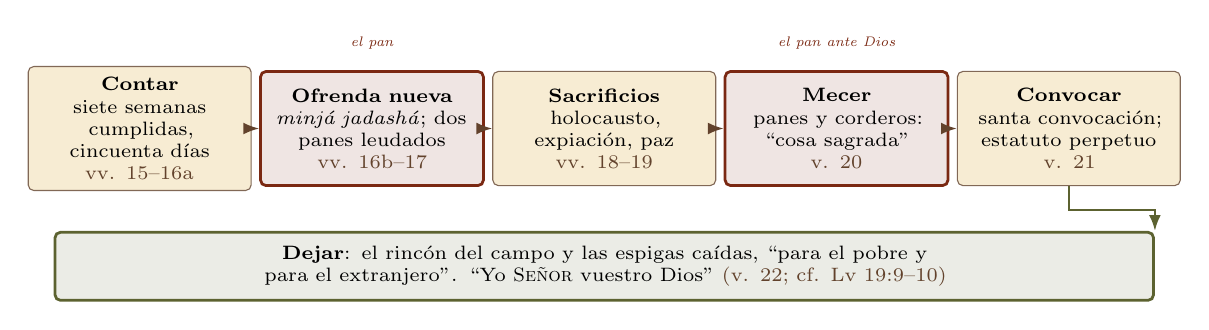
\begin{tikzpicture}[font=\scriptsize,
  bl/.style={draw=sepia!80,fill=papiro!70,rounded corners=2pt,text width=2.55cm,align=center,inner sep=4pt,minimum height=1.45cm},
  bc/.style={draw=tierraroja,line width=1pt,fill=tierraroja!12,rounded corners=2pt,text width=2.55cm,align=center,inner sep=4pt,minimum height=1.45cm}]
 \node[bl] (a) at (0,0) {\textbf{Contar}\\ siete semanas cumplidas, cincuenta días\\ {\color{sepia}vv. 15--16a}};
 \node[bc] (b) at (2.95,0) {\textbf{Ofrenda nueva}\\ \emph{minjá jadashá}; dos panes leudados\\ {\color{sepia}vv. 16b--17}};
 \node[bl] (c) at (5.9,0) {\textbf{Sacrificios}\\ holocausto, expiación, paz\\ {\color{sepia}vv. 18--19}};
 \node[bc] (d) at (8.85,0) {\textbf{Mecer}\\ panes y corderos: ``cosa sagrada''\\ {\color{sepia}v. 20}};
 \node[bl] (e) at (11.8,0) {\textbf{Convocar}\\ santa convocación; estatuto perpetuo\\ {\color{sepia}v. 21}};
 \node[draw=oliva,line width=1pt,fill=oliva!12,rounded corners=2pt,text width=13.6cm,align=center,inner sep=5pt] (f) at (5.9,-1.75) {\textbf{Dejar}: el rincón del campo y las espigas caídas, ``para el pobre y para el extranjero''. ``Yo \SENOR{} vuestro Dios'' {\color{sepia}(v. 22; cf. Lv 19:9--10)}};
 \foreach \u/\v in {a/b,b/c,c/d,d/e} \draw[-{Latex[length=2mm]},sepia,line width=0.7pt] (\u)--(\v);
 \draw[-{Latex[length=2mm]},oliva,line width=0.8pt] (e.south) |- ++(0,-0.3) -| (f.north east);
 \node[above=4pt of b.north,font=\tiny\itshape,text=tierraroja] {el pan};
 \node[above=4pt of d.north,font=\tiny\itshape,text=tierraroja] {el pan ante Dios};
\end{tikzpicture}\par
{\footnotesize\color{sepia}\textit{Figura 7.} Estructura de Lv 23:15--22: del tiempo contado al borde del campo. \textit{Nota.} Elaboración propia.}
\end{center}

Dos rasgos literarios distinguen el párrafo. El primero es la heptada: siete semanas, el séptimo sábado, siete corderos (v. 18), y la cifra cincuenta como ``siete más uno'' elevado a semanas. El segundo es el final. Todas las demás secciones de Levítico 23 terminan en el culto; esta termina en el campo, con una ley que el lector ya conoce por Lv 19:9--10. La repetición tiene una función: une la fiesta de la siega con el capítulo de la santidad (``santos seréis, porque santo soy yo'', Lv 19:2) y hace del borde del campo una parte de la liturgia.

\subsection{Sinaí y Hechos 2}

Lucas no cita Éxodo 19 en Hechos 2, pero su relato usa el vocabulario de la teofanía del Sinaí: un ruido del cielo, fuego visible, un pueblo reunido, una voz que todos entienden. Puestos uno junto al otro, los dos textos dejan ver hasta dónde llegan los paralelos.

\begin{center}
\begin{tikzpicture}[font=\scriptsize,
  iz/.style={draw=sepia!80,fill=papiro!70,rounded corners=2pt,text width=5.2cm,align=left,inner sep=3pt,minimum height=0.78cm},
  de/.style={draw=tierraroja,fill=tierraroja!8,rounded corners=2pt,text width=5.2cm,align=left,inner sep=3pt,minimum height=0.78cm},
  te/.style={font=\scriptsize\bfseries,text=caferojizo,text width=2.3cm,align=center}]
 \node[font=\small\bfseries,text=sepia] at (0,0.75) {Sinaí (Éx 19--20; 32)};
 \node[font=\small\bfseries,text=tierraroja] at (9.4,0.75) {Jerusalén (Hch 2)};
 \foreach \i/\t/\a/\b in {0/{Tiempo}/{``en el mes tercero'' tras la salida (19:1)}/{``al cumplirse el día de Pentecostés'' (2:1)},
   1/{Pueblo reunido}/{Moisés ``sacó del campamento al pueblo para recibir a Dios'' (19:17)}/{``estaban todos unánimes juntos'' (2:1)},
   2/{Descenso}/{``\SENOR{} había descendido sobre él en fuego'' (19:18)}/{``vino del cielo'' (2:2)},
   3/{Sonido}/{\emph{qolot}, ``voces''; \emph{qol shofar} muy fuerte (19:16; 20:18)}/{\grc{ἦχος}, ``estruendo''; \grc{φωνή}, ``voz'' (2:2, 6)},
   4/{Fuego}/{\emph{esh}, \emph{lapidim}: fuego y antorchas (19:18; 20:18)}/{\grc{γλῶσσαι ὡσεὶ πυρός} (2:3)},
   5/{La palabra}/{diez palabras; tablas ``escritas con el dedo de Dios'' (20:1; 31:18)}/{hablar ``las maravillas de Dios''; el Espíritu escribe en corazones (2:11; 2~Co 3:3)},
   6/{Tres mil}/{``como tres mil hombres'' mueren tras el becerro (32:28)}/{``como tres mil personas'' son añadidas (2:41)}}{
   \node[iz] (a\i) at (0,-\i*1.02) {\a};
   \node[de] (b\i) at (9.4,-\i*1.02) {\b};
   \node[te] at (4.7,-\i*1.02) {\t};
   \draw[mostaza!80!tierraroja,line width=0.6pt,dashed] (a\i.east) -- (3.5,-\i*1.02);
   \draw[mostaza!80!tierraroja,line width=0.6pt,dashed,-{Latex[length=1.8mm]}] (5.9,-\i*1.02) -- (b\i.west);}
\end{tikzpicture}\par
{\footnotesize\color{sepia}\textit{Figura 8.} Paralelos entre la teofanía del Sinaí y Hechos 2. \textit{Nota.} Elaboración propia con la RVR1960 y NA28. La última fila es un eco señalado por algunos intérpretes, no una cita.}
\end{center}

\begin{nota}[Precisión: el eco de los tres mil]
La correspondencia entre los tres mil que murieron después del becerro de oro (\heb{כִּשְׁלֹשֶׁת אַלְפֵי אִישׁ}, Éx 32:28) y los tres mil añadidos en Pentecostés (\grc{ψυχαὶ ὡσεὶ τρισχίλιαι}, Hch 2:41) aparece en lecturas tipológicas cristianas, incluida una de las fuentes del proyecto (Baker, 2013), que la resume con 2~Co 3:6: ``la letra mata, mas el espíritu vivifica''. Lucas no la señala, y el número de Hechos es aproximado (\grc{ὡσεί}). Es un eco posible, más fuerte si se acepta que Lucas narra Pentecostés con el Sinaí al fondo (§10).
\end{nota}

Una tradición judía antigua refuerza la lectura sinaítica de la Ascensión y de Pentecostés. El Salmo 68, que celebra la marcha de Dios desde el Sinaí al santuario (Sal 68:8, 17 [68:9, 18]), dice: ``Subiste a lo alto, cautivaste la cautividad, tomaste dones para los hombres'' (Sal 68:18 [68:19]). El Targum del Salmo aplica el versículo a Moisés, que subió al firmamento, aprendió las palabras de la Torá y las dio como dones a los hombres. Efesios cita el versículo con un cambio de verbo, ``dio dones a los hombres'', y lo aplica a Cristo que sube y reparte dones a su iglesia (Ef 4:8--11). Lincoln (1990) y Turner (1996) ven aquí la conexión Moisés--Cristo, Torá--Espíritu.

\begin{nota}[Precisión]
La autoría paulina de Efesios es discutida en la investigación; la carta se cita aquí como testimonio de la tradición paulina. La fecha del Targum de los Salmos es tardía, aunque puede conservar tradiciones antiguas. El argumento no depende de Efesios: el vínculo Espíritu--Ley escrita en el corazón aparece en 2~Co 3, carta indiscutida.
\end{nota}

\subsection{Del deseo de Moisés a la promesa de Joel}

En el desierto, Moisés se queja de que no puede cargar solo con el pueblo. Dios le manda reunir setenta ancianos, y ``tomó del espíritu que estaba en él, y lo puso en los setenta varones ancianos; y cuando posó sobre ellos el espíritu, profetizaron, y no cesaron'' (Nm 11:25). Dos de ellos, Eldad y Medad, profetizan en el campamento, fuera del tabernáculo, y Josué pide que se los impida. Moisés responde:

\needspace{5\baselineskip}\hebverso{וּמִי יִתֵּן כָּל־עַם יְהוָה נְבִיאִים כִּי־יִתֵּן יְהוָה אֶת־רוּחוֹ עֲלֵיהֶם}
\begin{cita}¿Tienes tú celos por mí? Ojalá todo el pueblo de \SENOR{} fuese profeta, y que \SENOR{} pusiera su espíritu sobre ellos.\fuente{(Nm 11:29)}\end{cita}

Joel convierte el deseo en promesa, y Pedro anuncia su cumplimiento:

\needspace{5\baselineskip}\hebverso{וְהָיָה אַחֲרֵי־כֵן אֶשְׁפּוֹךְ אֶת־רוּחִי עַל־כָּל־בָּשָׂר וְנִבְּאוּ בְּנֵיכֶם וּבְנוֹתֵיכֶם}
\begin{cita}Y después de esto derramaré mi Espíritu sobre toda carne, y profetizarán vuestros hijos y vuestras hijas; vuestros ancianos soñarán sueños, y vuestros jóvenes verán visiones. Y también sobre los siervos y sobre las siervas derramaré mi Espíritu en aquellos días.\fuente{(Jl 2:28--29 [3:1--2])}\end{cita}

\begin{center}
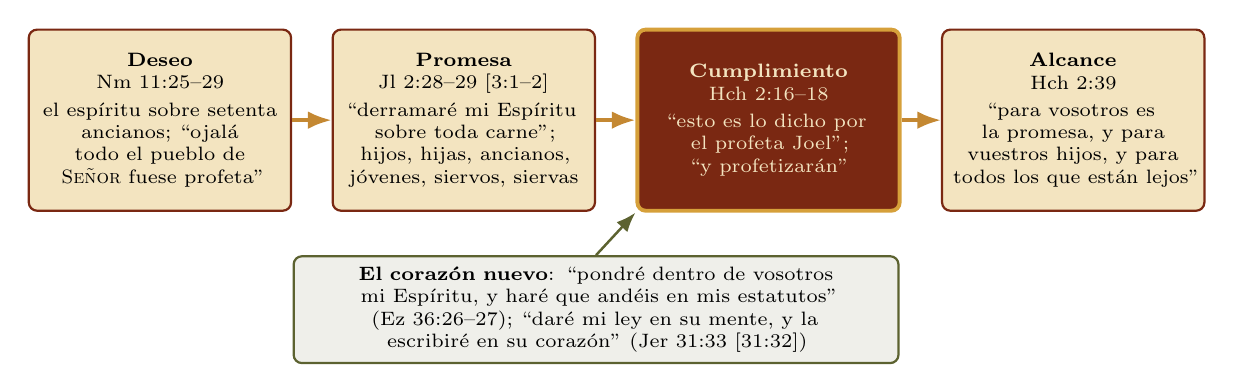
\begin{tikzpicture}[font=\scriptsize,node distance=0.5cm,
  bx/.style={draw=tierraroja,line width=0.8pt,fill=papiro,rounded corners=3pt,text width=3.05cm,align=center,inner sep=4pt,minimum height=2.3cm}]
 \node[bx] (n) {\textbf{Deseo}\\ Nm 11:25--29\\[2pt] el espíritu sobre setenta ancianos; ``ojalá todo el pueblo de \SENOR{} fuese profeta''};
 \node[bx,right=of n] (j) {\textbf{Promesa}\\ Jl 2:28--29 [3:1--2]\\[2pt] ``derramaré mi Espíritu sobre toda carne''; hijos, hijas, ancianos, jóvenes, siervos, siervas};
 \node[bx,right=of j,draw=mostaza,line width=1.4pt,fill=tierraroja,text=papiro] (h) {\textbf{Cumplimiento}\\ Hch 2:16--18\\[2pt] ``esto es lo dicho por el profeta Joel''; ``y profetizarán''};
 \node[bx,right=of h] (l) {\textbf{Alcance}\\ Hch 2:39\\[2pt] ``para vosotros es la promesa, y para vuestros hijos, y para todos los que están lejos''};
 \foreach \u/\v in {n/j,j/h,h/l} \draw[-{Latex[length=3mm]},mostaza!80!tierraroja,line width=1.3pt] (\u)--(\v);
 \node[draw=oliva,line width=0.8pt,fill=oliva!10,rounded corners=3pt,text width=7.4cm,align=center,inner sep=4pt,below=0.55cm of j.south east] (e) {\textbf{El corazón nuevo}: ``pondré dentro de vosotros mi Espíritu, y haré que andéis en mis estatutos'' (Ez 36:26--27); ``daré mi ley en su mente, y la escribiré en su corazón'' (Jer 31:33 [31:32])};
 \draw[-{Latex[length=2.5mm]},oliva,line width=0.9pt] (e.north) -- (h.south west);
\end{tikzpicture}\par
{\footnotesize\color{sepia}\textit{Figura 9.} La cadena profética del Espíritu: Números 11, Joel y Hechos 2. \textit{Nota.} Elaboración propia con la RVR1960.}
\end{center}

La lista de Joel recuerda la de Dt 16:11. En Shavuot se alegran ``tu hijo, tu hija, tu siervo, tu sierva''; en la promesa de Joel profetizan ``vuestros hijos y vuestras hijas'' y reciben el Espíritu ``los siervos y las siervas''. El paralelo es una observación mía y no una cita de Joel, pero sugiere que la fiesta que incluía a los de abajo en la alegría anticipa la promesa que los incluye en la profecía.

\subsection{Babel invertida}

Génesis 11 narra la dispersión de los pueblos por la confusión de una lengua: ``Ahora, pues, descendamos, y confundamos allí su lengua, para que ninguno entienda el habla de su compañero'' (Gn 11:7). La LXX traduce ``confundamos'' con \grc{συγχέωμεν}. En Hechos 2 la multitud de las naciones ``estaba confusa'' (\grc{συνεχύθη}, Hch 2:6), porque cada uno oía hablar en su propia lengua. El verbo es el mismo y la dirección es la contraria: en Babel la confusión dispersa; en Jerusalén reúne a los dispersos para que oigan lo mismo. Muchos comentaristas señalan el eco (Bruce, 1988; Keener, 2012); otros lo consideran posible, pero no programático, porque Lucas no cita Génesis 11 (Fitzmyer, 1998). En cualquier caso, Pentecostés no suprime la diversidad de lenguas sino que la pone al servicio del mensaje, y cada uno oye ``en su propia lengua''.

\subsection{La ley en el corazón: Jeremías, Ezequiel y 2 Corintios 3}

El vocabulario de Shavuot y el de la promesa del nuevo pacto se tocan en el adjetivo \emph{jadash}, ``nuevo'': la \emph{minjá jadashá} del grano nuevo (Lv 23:16), el \emph{brit jadashá} de Jer 31:31 y el \emph{lev jadash} y \emph{rúaj jadashá} de Ez 36:26. Jeremías define lo nuevo del pacto con la imagen de las tablas: la ley ya no se escribe en piedra sino en el corazón (Jer 31:33 [31:32]), y Ezequiel atribuye ese cambio al Espíritu: ``pondré dentro de vosotros mi Espíritu, y haré que andéis en mis estatutos'' (Ez 36:27).

Pablo une los dos textos al defender su ministerio ante los corintios:

\begin{cita}Siendo manifiesto que sois carta de Cristo expedida por nosotros, escrita no con tinta, sino con el Espíritu del Dios vivo; no en tablas de piedra, sino en tablas de carne del corazón.\fuente{(2~Co 3:3)}\end{cita}

``Tablas de piedra'' (\grc{πλαξὶν λιθίναις}) remite al Sinaí (Éx 31:18; 34:1); ``tablas de carne'' y ``corazón'' remiten a Ez 36:26 (``corazón de carne'') y a Jer 31:33 (Hays, 1989). En la misma carta Pablo llama a su servicio ``ministerio del espíritu'' frente al ``ministerio de muerte grabado con letras en piedras'' (2~Co 3:7--8). En Romanos describe el resultado: ``la ley del Espíritu de vida en Cristo Jesús me ha librado de la ley del pecado y de la muerte\ldots{} para que la justicia de la ley se cumpliese en nosotros'' (Ro 8:2, 4). El mismo capítulo recurre al lenguaje de la siega cuando dice que los creyentes ``tenemos las primicias del Espíritu'' (\grc{τὴν ἀπαρχὴν τοῦ πνεύματος}, Ro 8:23), un anticipo de la cosecha completa.

\begin{nota}[Precisión]
Pablo no menciona Shavuot en 2~Co 3 ni en Ro 8. El vínculo entre la fiesta y estos textos es temático (Sinaí, tablas, Espíritu, primicias) y se apoya en la asociación judía de la fiesta con el pacto (§3). Es una lectura canónica legítima, coherente con el principio de la serie de que la Biblia interpreta la Biblia, pero no una afirmación explícita de Pablo.
\end{nota}

%===================================================================
\section{Memorial, figura y esperanza: la lectura de la serie}

\subsection{El marco}

El documento de referencia de la serie lee Levítico 23 como el ``Reglamento del Culto'' de Dios: las solemnidades del \SENOR{} proclamadas como convocaciones santas ``en sus tiempos'', estatuto perpetuo, distintas de ``la ley de los sacrificios'' que las acompaña (Nm 28--29). Divide la historia del pueblo de Dios en tres períodos: la Congregación de los Primogénitos (de Adán a Abraham), Israel como congregación del desierto (Hch 7:38) y la Iglesia del Nuevo Pacto. Cada fiesta es a la vez \destacar{memorial} de un hito histórico de Israel y \destacar{figura} de una etapa del plan de salvación. Para Shavuot, el documento resume:

\begin{cita}La Fiesta de la Siega ---> La manifestación del Espíritu de Dios en el Monte Sinaí, y la Data de la Ley.\fuente{(Documento de la serie, lección 7)}\end{cita}

Y enumera tres rasgos de la fiesta: instituida ``para conmemorar el día de la data de la Ley''; ``mandato de carácter perpetuo''; y ``el día de Pentecostés se debe declarar sábado santo''.

\begin{center}\small\renewcommand{\arraystretch}{1.25}
\begin{tabular}{@{}L{3.6cm}L{3.2cm}L{8.6cm}@{}}
\toprule
\textbf{Hito de Israel} & \textbf{Fiesta} & \textbf{Nuevo Pacto (lectura de la serie)} \\ \midrule
Manifestación en el Sinaí y entrega de la Ley (Éx 19--20) & Pentecostés, Siega, Semanas & Derramamiento del Espíritu (Hch 2); dos panes con levadura (Lv 23:17) = pueblos aún con pecado considerados para la redención; lluvias de Joel 2:23: primera, temprana, tardía y ``del principio'' \\
\bottomrule
\end{tabular}\par
{\footnotesize\color{sepia}\textit{Tabla 4.} Shavuot en el esquema de la serie. \textit{Nota.} Resumen del documento de referencia (lecciones 7, 9 y 11).}
\end{center}

\subsection{El memorial: el Sinaí}

El documento ubica Shavuot en la secuencia de la salida de Egipto: Israel salvado de la muerte (Pascua), libre del cautiverio (Ázimos), primicia de las naciones tras cruzar el mar (\emph{ómer}), y la ``manifestación de Dios en el Sinaí'' con la entrega de la Ley (Siega). La lectura histórica (§3.5) mostró que la cronología de Éx 19:1 admite esa conexión y que el judaísmo del Segundo Templo ya la hacía (Jubileos, Qumrán), aunque la Torá no la formula. La tesis de la serie queda en buen terreno si se la presenta como lectura del calendario a la luz de la historia, y no como texto explícito.

El documento ve una anticipación de Pentecostés en la vida de Abraham: ``la manifestación de Dios en una lengua de fuego, a la semejanza de la manifestación de Pentecostés, cuando Abraham moraba en Mamre'' (lección 6). El texto bíblico más cercano es el pacto entre los animales partidos, donde ``un horno humeando, y una antorcha de fuego que pasaba por entre los animales divididos'' (Gn 15:17) sella la promesa. Abram habitaba entonces en el encinar de Mamre (Gn 13:18; 14:13).

\begin{nota}[Precisión]
Gn 15:17 dice \heb{לַפִּיד אֵשׁ} (\emph{lapid esh}), ``antorcha de fuego'', no ``lengua de fuego''. La palabra \emph{lapid} es la misma de las ``antorchas'' del Sinaí (\heb{לַפִּידִם}, Éx 20:18), y el humo del horno recuerda el humo del monte ``como el humo de un horno'' (Éx 19:18). El vínculo léxico Gn 15--Éx 19--20 es real; el vínculo con las lenguas de Hch 2 es tipológico. Ambos pueden aceptarse, con esa diferencia de grado: lo primero es filológico, lo segundo, figura.
\end{nota}

\begin{nota}[Precisión: ¿``sábado santo''?]
Lv 23:21 llama a Shavuot \emph{mikrá kódesh} (santa convocación) y prohíbe ``trabajo de siervos'' (\heb{כָּל־מְלֶאכֶת עֲבֹדָה}). A diferencia de Yom Teruá, Yom Kipur y Sukkot (Lv 23:24, 32, 39), el texto no lo llama \emph{shabat} ni \emph{shabatón}. La expresión del documento (``se debe declarar sábado santo'') es correcta si se entiende como día de reposo festivo y convocación; no es un sábado semanal.
\end{nota}

\subsection{La figura: el Espíritu derramado}

La lección 11 del documento formula la pregunta que recorre toda la serie: el Espíritu fue derramado ``con motivo de esta Solemnidad'', cuando el Señor ya había resucitado y vuelto al Padre. ``¿Cómo pudo manifestarse el Espíritu sobre ellos si estaban celebrando una Fiesta, presuntamente obsoleta a causa de la muerte de Cristo en la cruz?'' El documento lo toma como indicio de que Dios ``se gratificaba con lo que la Iglesia estaba haciendo'' (lección 9), y añade un dato de calendario: el derramamiento ocurrió ``diez días después del retorno del Señor Jesús a la diestra de su Padre'', porque Jesús se apareció durante cuarenta días (Hch 1:3) y Pentecostés es el día cincuenta.

La lectura sigue la lógica interna de la serie. Si el \emph{ómer} es Cristo, primicia de los resucitados, recibido a la diestra del Padre (1~Co 15:20--23), los cincuenta días llevan de la primicia a la cosecha, y el día cincuenta es aquel en que la primicia ascendida envía el Espíritu. Pedro mismo hace la conexión: ``exaltado por la diestra de Dios, y habiendo recibido del Padre la promesa del Espíritu Santo, ha derramado esto que vosotros veis y oís'' (Hch 2:33).

\subsection{Los dos panes con levadura}

La lección 11 dedica su argumento central a los dos panes. Conviene citarla en sus propias palabras:

\begin{cita}En el periodo del Primer Pacto el Reglamento de Culto, junto con determinar el momento de celebrar la Fiesta de Pentecostés, exigía la presentación de dos panes, en calidad de Ofrenda Mecida por Primicias a Dios; los que no teniendo la finalidad de ser presentes expiatorios, cumplían la función de prefigurar simbólicamente una parte importante del Plan de Dios para con la humanidad.\fuente{(Documento de la serie, lección 11)}\end{cita}

Lo particular está en la levadura. ``La misma Ley prohibía terminantemente el uso de la levadura en ofrendas y sacrificios''; la excepción es ``una sombra precursora'' de algo que ``ni aún los santos hombres del pasado pudieron descifrar'', reservado, según Ef 3:1--6, ``para el conocimiento de la Iglesia''. El documento recorre luego la serie de figuras: el cordero de Pascua es Cristo; la masa sin levadura de Ázimos es ``la marcha de la Iglesia liberada de la levadura del pecado''; el \emph{ómer} representa ``al Señor Jesús, en una nueva función tras ser recibido en el cielo a la diestra de Dios''. Y para los panes recuerda las tres etapas de la historia de la Iglesia, que lee en Mt 13:33 (la levadura escondida en tres medidas de harina):

\begin{cita}El Apóstol Pablo en la Carta a los Hebreos (Cáp. 12:22--24) declara que ya la Congregación de los Primogénitos está alistada en los cielos, pues sus nombres ya están inscritos en el Libro de la Vida, esto lo dice en alusión a todos aquellos fieles que fueron desde Adán hasta el Pacto de Dios con Abraham. Sin embargo, falta todavía que la salvación de Israel sea consumada, lo que sucederá cuando se haya integrado al Pueblo de Dios la plenitud de los gentiles. Estos dos estamentos, a pesar de su pecado, están considerados delante de Dios para el momento de su redención y representados simbólicamente en estos ``dos panes con levadura'' que exigía para este día la Ley.\fuente{(Documento de la serie, lección 11)}\end{cita}

El núcleo de la tesis se entiende bien: los panes llevan levadura porque representan a pueblos que todavía tienen pecado, pero que Dios ya ``considera'' para la redención; son ``primicias'' porque pertenecen a Dios antes de la cosecha completa. Menos claro es quiénes son los ``dos estamentos'', porque el propio párrafo admite dos lecturas. Si se toma el antecedente más cercano, son \destacar{Israel}, cuya salvación ``falta todavía'' consumar, y \destacar{la plenitud de los gentiles} que debe integrarse al pueblo de Dios (cf. Ro 11:25--26). Si se toma el párrafo completo, el primer término es la \destacar{Congregación de los Primogénitos}, ya inscrita en los cielos, y el segundo, \destacar{Israel} con los gentiles que se le integran. El documento no resuelve la ambigüedad; en ambos casos distingue los dos panes de Cristo (el \emph{ómer}) y de la Iglesia sin levadura (Ázimos).

\begin{center}
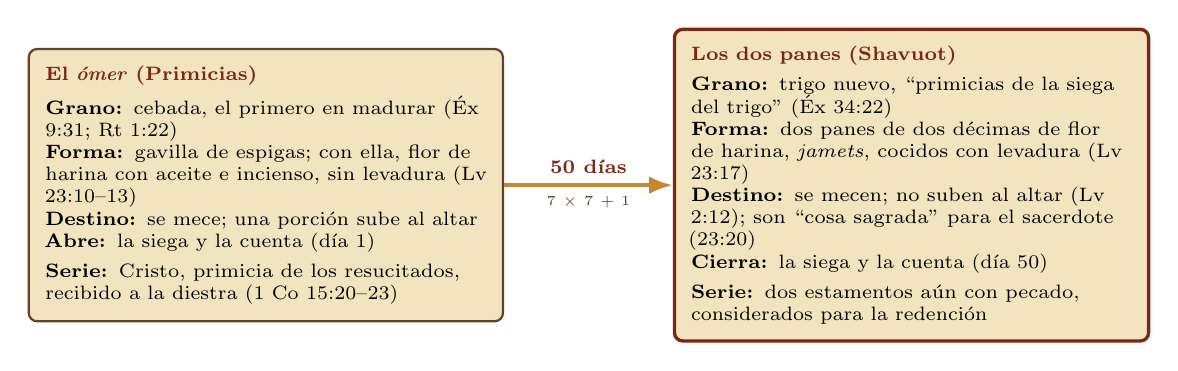
\begin{tikzpicture}[font=\scriptsize,
  co/.style={draw=sepia,line width=0.8pt,fill=papiro,rounded corners=3pt,text width=5.6cm,align=left,inner sep=6pt}]
 \node[co] (o) at (0,0) {\textbf{\color{tierraroja}El \emph{ómer} (Primicias)}\\[3pt]
  \textbf{Grano:} cebada, el primero en madurar (Éx 9:31; Rt 1:22)\\
  \textbf{Forma:} gavilla de espigas; con ella, flor de harina con aceite e incienso, sin levadura (Lv 23:10--13)\\
  \textbf{Destino:} se mece; una porción sube al altar\\
  \textbf{Abre:} la siega y la cuenta (día 1)\\[3pt]
  \textbf{Serie:} Cristo, primicia de los resucitados, recibido a la diestra (1~Co 15:20--23)};
 \node[co,draw=tierraroja,line width=1.2pt] (p) at (8.2,0) {\textbf{\color{tierraroja}Los dos panes (Shavuot)}\\[3pt]
  \textbf{Grano:} trigo nuevo, ``primicias de la siega del trigo'' (Éx 34:22)\\
  \textbf{Forma:} dos panes de dos décimas de flor de harina, \emph{jamets}, cocidos con levadura (Lv 23:17)\\
  \textbf{Destino:} se mecen; no suben al altar (Lv 2:12); son ``cosa sagrada'' para el sacerdote (23:20)\\
  \textbf{Cierra:} la siega y la cuenta (día 50)\\[3pt]
  \textbf{Serie:} dos estamentos aún con pecado, considerados para la redención};
 \draw[-{Latex[length=3mm]},mostaza!80!tierraroja,line width=1.4pt] (o.east) -- node[above,font=\scriptsize\bfseries,text=tierraroja]{50 días} node[below,font=\tiny,text=sepia]{7 $\times$ 7 + 1} (p.west);
\end{tikzpicture}\par
{\footnotesize\color{sepia}\textit{Figura 10.} El \emph{ómer} de cebada y los dos panes de trigo: los dos extremos de la cuenta. \textit{Nota.} Elaboración propia con la RVR1960 y el documento de la serie (lección 11).}
\end{center}

\begin{nota}[Precisiones a la lectura de los dos panes]
\textbf{(1)} La prohibición general de la levadura en el altar está en Lv 2:11; el documento cita Lv 2:4--5, que la aplica a las tortas cocidas. El mismo capítulo prevé la excepción de las primicias leudadas, que ``no subirán sobre el altar'' (Lv 2:12); la ley no se contradice, separa lo que va al fuego de lo que se mece y se entrega. \textbf{(2)} El documento atribuye Hebreos a Pablo; la autoría de Hebreos es discutida desde la Iglesia antigua y la carta no nombra a su autor (Attridge, 1989; Lane, 1991). El argumento de la serie se apoya en el contenido de He 12:22--24 (``la congregación de los primogénitos que están inscritos en los cielos''), no en su autor. \textbf{(3)} También Efesios es de autoría discutida; Ef 3:6 (``los gentiles son coherederos y miembros del mismo cuerpo'') tiene paralelo en cartas indiscutidas (Ro 11:17--24; Gá 3:28). \textbf{(4)} La levadura no siempre simboliza el pecado en la Escritura: en 1~Co 5:6--8, Gá 5:9 y Mt 16:6 sí; en Mt 13:33 (el texto que el documento usa para las tres etapas) es figura del reino que crece. \textbf{(5)} La interpretación de los dos panes es tipológica; Levítico no la explica.
\end{nota}

\subsection{Las lluvias de Joel 2:23}

La lección 11 continúa con el sermón de Pedro (``esto es lo dicho por el profeta Joel'', Hch 2:16) y lee el versículo de Joel que precede a la promesa del Espíritu, en la versión de 1909: ``os ha dado la primera lluvia arregladamente, y hará descender sobre vosotros lluvia temprana y tardía como al principio'' (Jl 2:23). De ahí distingue cuatro lluvias:

\begin{cita}``La primera lluvia arregladamente''. El Espíritu Santo estuvo presente en la conducción de la nación, más no siempre, ni en todos. ``La Lluvia Temprana'', por su parte, corresponde a la manifestación del Santo Espíritu, en el Aposento Alto, extensiva para la Iglesia del Nuevo Pacto. ``La Lluvia del Principio'', entre tanto, alude la innegable presencia del Espíritu en la Congregación de los Primogénitos, en donde Dios se manifestaba cara a cara a sus Hijos. ``La Lluvia Tardía'', finalmente, tiene que ver con la promesa de la manifestación del Espíritu Santo, en el tiempo del fin a la Nación del Pacto; cuando definitivamente la venda de sus ojos sea quitada al mismo tiempo que haya entrado el último de los gentiles al pueblo de Dios.\fuente{(Documento de la serie, lección 11)}\end{cita}

\begin{center}
\begin{tikzpicture}[font=\scriptsize,
  rb/.style={draw=oliva,line width=0.8pt,fill=oliva!10,rounded corners=3pt,text width=3.25cm,align=center,inner sep=4pt,minimum height=1.55cm},
  sb/.style={draw=tierraroja,line width=0.8pt,fill=papiro,rounded corners=3pt,text width=3.25cm,align=center,inner sep=4pt,minimum height=1.55cm}]
 \node[font=\scriptsize\bfseries,text=oliva!70!black,anchor=west] at (-1.9,1.25) {Jl 2:23 (orden del versículo)};
 \foreach \i/\h/\t/\f in {0/{\heb{הַמּוֹרֶה לִצְדָקָה}}/{``la primera lluvia arregladamente''}/{lluvia o maestro (§4)},1/{\heb{מוֹרֶה}}/{``lluvia temprana''}/{otoño: \emph{yoré}},2/{\heb{מַלְקוֹשׁ}}/{``tardía''}/{primavera},3/{\heb{בָּרִאשׁוֹן}}/{``como al principio''}/{adverbio: ``en el primero''}}{
   \node[rb] (r\i) at (\i*3.85,0) {\large\h\\[1pt] \scriptsize\t\\ {\tiny\color{sepia}\f}};}
 \foreach \i/\s in {0/{El Espíritu en algunos de Israel: sacerdotes, profetas, reyes; ``no siempre, ni en todos''},1/{El Aposento Alto (Hch 2), extendido a la Iglesia del Nuevo Pacto},2/{Israel en el tiempo del fin, cuando entre el último de los gentiles},3/{La Congregación de los Primogénitos: Dios ``cara a cara''}}{
   \node[sb] (s\i) at (\i*3.85,-2.15) {\s};
   \draw[-{Latex[length=2mm]},sepia,line width=0.7pt] (r\i.south) -- (s\i.north);}
 \node[font=\scriptsize\bfseries,text=tierraroja,anchor=west] at (-1.9,-3.65) {Orden histórico según la serie};
 \draw[line width=1.4pt,tierraroja,-{Latex[length=3mm]}] (-1.7,-4.7) -- (13.4,-4.7);
 \foreach \x/\t/\c in {-0.6/{1. Primogénitos}/{``del principio''},3.3/{2. Israel}/{``la primera, arregladamente''},7.2/{3. Iglesia}/{``temprana''},11.1/{4. Israel al fin}/{``tardía''}}{
   \fill[mostaza] (\x+0.6,-4.7) circle (3.5pt);
   \node[above=4pt,font=\scriptsize\bfseries,text=caferojizo] at (\x+0.6,-4.7) {\t};
   \node[below=4pt,font=\tiny,text=sepia] at (\x+0.6,-4.7) {\c};}
\end{tikzpicture}\par
{\footnotesize\color{sepia}\textit{Figura 11.} Las cuatro lluvias de Joel 2:23 según la serie: el texto hebreo, su lectura y su orden histórico. \textit{Nota.} Elaboración propia con la BHS, la RV 1909 y el documento de la serie (lección 11).}
\end{center}

El punto de partida de esta lectura tiene apoyo textual firme, porque Joel pasa de la lluvia al Espíritu sin cambiar de imagen: ``hará descender sobre vosotros lluvia'' (v. 23) y ``derramaré mi Espíritu'' (\heb{אֶשְׁפּוֹךְ}, 3:1) están unidos por ``después de esto''. Isaías hace la misma equivalencia: ``Porque yo derramaré aguas sobre el sequedal, y ríos sobre la tierra árida; mi Espíritu derramaré sobre tu generación'' (Is 44:3), y Oseas compara la venida de Dios con ``la lluvia tardía y temprana a la tierra'' (Os 6:3). Leer las lluvias como figuras del Espíritu es seguir una metáfora de los propios profetas.

\begin{nota}[Precisión filológica: cuatro lluvias, dos palabras]
\textbf{(1)} En hebreo el versículo nombra dos tipos de lluvia: \emph{moré} (= \emph{yoré}), la temprana de otoño, y \emph{malqosh}, la tardía de primavera. ``La primera lluvia arregladamente'' traduce \emph{hamoré litsdaká}, que es la misma palabra \emph{moré} con artículo (o ``el maestro de justicia''); y ``como al principio'' traduce \emph{barishón}, un adverbio de tiempo (``en el primero'', ``como antes''), no una cuarta lluvia. La serie construye cuatro figuras sobre la traducción castellana; en hebreo hay dos lluvias, un \emph{moré} discutido y una indicación temporal. \textbf{(2)} En el año agrícola, la lluvia temprana cae en otoño, al sembrar, y la tardía en primavera, antes de la siega; Shavuot cae en la estación seca. La serie usa ``temprana'' y ``tardía'' en sentido de secuencia histórica (primero y último), no de estación. \textbf{(3)} La identificación de cada lluvia con una etapa (Primogénitos, Israel, Iglesia, Israel al fin) es interpretación de la serie; otros movimientos han leído la ``lluvia tardía'' como un derramamiento final del Espíritu sobre la Iglesia (así el pentecostalismo temprano: Myland, 1910). Ninguna de estas identificaciones está en Joel ni en Hechos.
\end{nota}

\subsection{Shavuot y el pacto matrimonial}

En mi presentación anterior propuse una figura más: Shavuot como \destacar{boda entre el Mesías (el novio) e Israel (la novia)}, en dos etapas, como el matrimonio judío antiguo. Primero el compromiso (\emph{erusín} o \emph{kidushín}), un contrato que deja a los novios legalmente casados sin cohabitar todavía; después la boda (\emph{nisuín}), cuando el novio lleva a la novia a su casa.

La figura se apoya en el lenguaje de los profetas, que describen el pacto del Sinaí como un matrimonio. Jeremías recuerda ``el amor de tu desposorio, cuando andabas en pos de mí en el desierto'' (Jer 2:2), y define el pacto roto con la misma imagen: ``porque ellos invalidaron mi pacto, aunque fui yo un marido para ellos'' (Jer 31:32 [31:31]). Oseas anuncia la renovación: ``Y te desposaré conmigo para siempre; te desposaré conmigo en justicia, juicio, benignidad y misericordia. Y te desposaré conmigo en fidelidad, y conocerás a \SENOR'' (Os 2:19--20 [2:21--22]). Éxodo 19--24 tiene la forma de ese pacto: la propuesta (``vosotros me seréis un reino de sacerdotes'', 19:5--6), el consentimiento del pueblo (``todo lo que \SENOR{} ha dicho, haremos'', 19:8; 24:3, 7), el documento escrito (24:4, 7) y la comida ante Dios (24:11). La tradición judía hizo explícita la imagen: la Misná lee ``el día de su desposorio'' del Cantar (Cnt 3:11) como ``la entrega de la Torá'' (m. Taanit 4:8).

En el Nuevo Testamento, Pablo describe la relación de Cristo con la iglesia como la del esposo con la esposa (Ef 5:25--32; cf. 2~Co 11:2, ``os he desposado con un solo esposo''), y el Apocalipsis anuncia la boda futura: ``han llegado las bodas del Cordero, y su esposa se ha preparado'' (Ap 19:7--9). Leída así, Shavuot correspondería al compromiso, con el pacto escrito en el Sinaí y el Espíritu como prenda en Pentecostés (§8.5), mientras la boda queda para el final.

\begin{nota}[Precisión]
La lectura de Shavuot como compromiso matrimonial es tipológica. Su base es real: los profetas describen el pacto como desposorio (Jer 2:2; 31:32; Os 2:19--20) y la Misná asocia el ``desposorio'' de Cnt 3:11 con la entrega de la Torá. Pero ningún texto bíblico llama a Shavuot ``boda'' ni ``compromiso'', y las dos etapas del matrimonio (\emph{erusín} y \emph{nisuín}) se conocen por la legislación rabínica posterior. Efesios es de autoría discutida; 2~Co 11:2 da la imagen en una carta indiscutida.
\end{nota}

\subsection{Pentecostés guardado por la Iglesia apostólica}

El documento concluye que la Iglesia de los apóstoles guardaba la fiesta: los discípulos estaban ``todos unánimes juntos'' el día de Pentecostés (Hch 2:1); Pablo se apresuraba ``por estar el día de Pentecostés, si le fuese posible, en Jerusalén'' (Hch 20:16); y escribe a Corinto desde Éfeso: ``estaré en Éfeso hasta Pentecostés'' (1~Co 16:8), ``lo cual señala que esta Iglesia gentil, también guardaba esta Fiesta de Adoración'' (lección 9). El folleto de la Iglesia de Dios Unida cita los mismos textos y el comentario de \emph{The Expositor's Bible Commentary}, según el cual Pablo quería llegar a Jerusalén ``para [la Fiesta de] Pentecostés en el quincuagésimo día después de la Pascua'' (Iglesia de Dios Unida, 2011).

\begin{nota}[Precisión]
Los tres textos muestran que la fiesta seguía siendo un punto fijo del calendario de los apóstoles; lo que se discute es su alcance. Hch 20:16 indica un viaje de peregrinación a Jerusalén; 1~Co 16:8 puede leerse como observancia de la fiesta en Éfeso, como sostiene la serie, o como simple referencia de calendario para fijar la fecha de un viaje, como prefieren otros comentaristas (Fee, 1987). Ninguno de los textos describe cómo se celebraba la fiesta en una iglesia de gentiles.
\end{nota}

%===================================================================
\section{Shavuot en Jesús y los apóstoles}

\subsection{La promesa del Padre}

Los evangelios no narran ninguna celebración de Shavuot en la vida de Jesús, pero el final de Lucas y el comienzo de Hechos orientan todo hacia ella. El Resucitado manda a los discípulos quedarse en Jerusalén ``hasta que seáis investidos de poder desde lo alto'' (Lc 24:49) y les recuerda ``la promesa del Padre'': ``vosotros seréis bautizados con el Espíritu Santo dentro de no muchos días'' (Hch 1:4--5). La espera dura lo que falta de la cuenta, pues Jesús se aparece ``durante cuarenta días'' (Hch 1:3) y el Espíritu llega ``al cumplirse el día de Pentecostés''. El Evangelio de Juan narra un don del Espíritu el mismo día de la resurrección (``Recibid el Espíritu Santo'', Jn 20:22); los intérpretes discuten si se trata de una anticipación del don de Pentecostés o de la versión joánica del mismo acontecimiento.

\subsection{La siega como misión}

Jesús usa el lenguaje de la siega para describir su misión. ``A la verdad la mies es mucha, mas los obreros pocos. Rogad, pues, al Señor de la mies, que envíe obreros a su mies'' (Mt 9:37--38). En Samaria dice: ``Alzad vuestros ojos y mirad los campos, porque ya están blancos para la siega'' (Jn 4:35), y distingue a quien siembra de quien siega (4:36--38). La palabra griega es \grc{θερισμός}, la que la LXX usa para \emph{qatsir} (Éx 34:22, \grc{θερισμοῦ πυρῶν}, ``siega del trigo''). Pentecostés, con tres mil personas añadidas en un día, es la primera siega abundante de esa misión.

\begin{nota}[Precisión]
Una de las fuentes del proyecto relaciona la ley de Lv 23:22 con los discípulos que arrancaban espigas en sábado (Mt 12:1; Baker, 2013). La ley que autoriza el gesto es otra: ``Cuando entres en la mies de tu prójimo, podrás arrancar espigas con tu mano; mas no aplicarás hoz a la mies de tu prójimo'' (Dt 23:25 [23:26]). La discusión de Mt 12 es sobre el sábado, no sobre la \emph{peá}.
\end{nota}

\subsection{Hechos 2: Pedro lee la fiesta}

El discurso de Pedro (Hch 2:14--36) tiene tres partes: la explicación del fenómeno con Joel (vv. 14--21), el anuncio de Jesús crucificado y resucitado con el Salmo 16 (vv. 22--32) y la exaltación con el Salmo 110 (vv. 33--36). La conclusión une las tres: el que fue resucitado y exaltado ``ha derramado esto que vosotros veis y oís'' (v. 33). El pueblo responde con la pregunta de la conversión, ``¿qué haremos?'', y Pedro contesta con el arrepentimiento, el bautismo y la promesa: ``para vosotros es la promesa, y para vuestros hijos, y para todos los que están lejos'' (vv. 37--39). Lucas cierra con la vida de la comunidad, que perseveraba en la doctrina de los apóstoles, la comunión, el partimiento del pan y las oraciones, ``y perseverando unánimes cada día en el templo'' (vv. 42, 46).

La escena reúne en un solo día los temas de la fiesta: la siega (tres mil), el pueblo reunido de la diáspora, la palabra que todos oyen, y la alegría que Deuteronomio mandaba, pues ``comían juntos con alegría y sencillez de corazón'' (Hch 2:46).

\subsection{Pablo: primicias del Espíritu}

Pablo no narra Pentecostés, pero su lenguaje sobre el Espíritu usa las categorías de la fiesta. Los creyentes tienen ``las primicias del Espíritu'' y esperan ``la redención de nuestro cuerpo'' (Ro 8:23): la primicia ya está en la mano, la cosecha todavía no. El Espíritu es ``las arras'' de la herencia (2~Co 1:22; 5:5), y la ley escrita en el corazón por el Espíritu reemplaza las tablas de piedra (2~Co 3:3--8). En Romanos 11, al hablar de Israel, Pablo usa la imagen del pan de las primicias: ``Si las primicias son santas, también lo es la masa'' (Ro 11:16), con una alusión a la ofrenda de la primera masa de Nm 15:19--21. En el mismo capítulo, Israel y los gentiles son ramas de un solo olivo (11:17--24), y ``todo Israel será salvo'' cuando haya entrado ``la plenitud de los gentiles'' (11:25--26), el texto que el documento de la serie supone al hablar de los dos estamentos.

\subsection{Las arras del Espíritu}

En mi presentación anterior destaqué la palabra con que Pablo nombra el don del Espíritu: \grc{ἀρραβών} (\emph{arrabōn}; Strong G728), ``arras'', ``prenda''. En el comercio griego era el pago adelantado que garantizaba una compra; si la compra no se efectuaba, quien había dado las arras las perdía. La palabra es un préstamo semítico, del hebreo \heb{עֵרָבוֹן} (\emph{eravón}), ``prenda'', de la raíz \heb{ערב}, ``salir fiador''. La Septuaginta la conserva en el único relato donde aparece: Judá deja a Tamar su sello, su cordón y su báculo como \emph{eravón} hasta enviarle el cabrito prometido (Gn 38:17--18, 20; LXX \grc{ἀρραβών}).

\begin{cita}El cual también nos ha sellado, y nos ha dado las arras del Espíritu en nuestros corazones.\fuente{(2~Co 1:22)}\end{cita}

Pablo lo repite en 2~Co 5:5 y Efesios lo desarrolla: ``fuisteis sellados con el Espíritu Santo de la promesa, que es las arras de nuestra herencia hasta la redención de la posesión adquirida'' (Ef 1:13--14). En griego moderno \emph{arrabōna} significa ``compromiso matrimonial'' y designa también el anillo de compromiso. El dato moderno no determina el sentido de Pablo, pero muestra el camino que recorrió la palabra, de la prenda comercial a la prenda nupcial. Leído junto a Ro 8:23, el sentido coincide con el de Shavuot: el Espíritu es la primicia y la prenda, y la cosecha y la boda vienen después.

\subsection{Santiago y Apocalipsis}

Santiago aplica el lenguaje de la siega a la espera de la venida del Señor: ``Mirad cómo el labrador espera el precioso fruto de la tierra, aguardando con paciencia hasta que reciba la lluvia temprana y la tardía'' (Stg 5:7), y llama a los creyentes ``primicias de sus criaturas'' (Stg 1:18). El Apocalipsis llama a los ciento cuarenta y cuatro mil ``primicias para Dios y para el Cordero'' (Ap 14:4) y describe a continuación dos siegas: la de la tierra y la de la vendimia (14:14--20). El paso de las primicias a la cosecha final, que Levítico 23 inscribe en el año, el Nuevo Testamento lo convierte en un paso de la historia. En mi presentación anterior reuní los textos proféticos de la cosecha: la fiesta de la cosecha de otoño (Dt 16:13), la tierra asolada y la siega del juicio (Is 24:1--7; 32:1--13), el que pisa el lagar (Is 63:1--9; Ap 19:11--15) y la vendimia de la tierra (Ap 14:18--20). Todos pertenecen a la siega final y a la vendimia, que el calendario sitúa en otoño; Shavuot corresponde a la siega intermedia, la de las primicias del trigo.

%===================================================================
\section{Shavuot en la tradición judía}

Lo que sigue es tradición judía posterior a la Biblia. Se expone para ver cómo Israel leyó la fiesta; no obliga a la lectura cristiana ni a la de la serie.

\subsection{\emph{Atséret}: la clausura de Pésaj}

La Misná y Josefo llaman a la fiesta \heb{עֲצֶרֶת} (\emph{atséret}; arameo \emph{Asartha}), ``asamblea de clausura'' (m. Rosh Hashaná 1:2; m. Bikurim 1:3; Josefo, \emph{Ant.} 3.252). El término es el que la Biblia usa para el octavo día de Sukkot (Lv 23:36; Nm 29:35). Shavuot aparece así como el cierre de Pésaj, igual que el octavo día cierra Sukkot, y las siete semanas forman una sola temporada que va de la salida de Egipto a la siega del trigo.

\subsection{El templo: primicias y panes}

La Misná describe la procesión de las primicias hacia Jerusalén: los de cada distrito se reunían en la ciudad principal, subían con un buey adornado delante, al son de la flauta, y eran recibidos por los artesanos de Jerusalén (m. Bikurim 3:2--4). Las primicias no podían traerse antes de Atséret (m. Bikurim 1:3), y desde entonces hasta Sukkot se recitaba la confesión de Dt 26:5--10 (``Un arameo a punto de perecer fue mi padre''). Para los dos panes, la Misná fija las medidas (siete palmos de largo, cuatro de ancho, con ``cuernos'' de cuatro dedos; m. Menajot 11:4) y añade que se amasaban y cocían por separado (m. Menajot 11:1). El grano nuevo no podía ofrecerse en el templo antes de los dos panes (m. Menajot 10:6).

\subsection{El tiempo de la entrega de la Torá}

Con el calendario fijo, la tradición rabínica estableció Shavuot el 6 de Siván y en la diáspora agregó un segundo día. El Talmud discute la fecha del Sinaí (b. Shabbat 86b) y afirma que Atséret es ``el día en que fue dada la Torá'' (b. Pesajim 68b); la liturgia posterior llama a la fiesta \emph{zman matán toratenu}. Para las lecturas, el Talmud prescribe ``Siete semanas'' (Dt 16:9) con Habacuc 3 como \emph{haftará} o, según otros, ``en el mes tercero'' (Éx 19) con la visión del carro de Ezequiel 1 (b. Meguilá 31a). Otra tradición talmúdica dice que cada palabra que salía de la boca de Dios en el Sinaí se dividía en setenta lenguas (b. Shabbat 88b; cf. \emph{Éxodo Rabá} 5:9). La imagen recuerda Hechos 2, aunque la fuente es varios siglos posterior.

\subsection{Las tres trompetas}

En mi presentación recogí una asociación judía de tres toques de \emph{shofar}. El primero, en el Sinaí: ``el sonido de la bocina iba aumentando en extremo'' (Éx 19:19), que la tradición sitúa en Shavuot. El último, el de Yom Teruá, que Pablo relaciona con ``la final trompeta'' de la resurrección (1~Co 15:51--53). Y la ``gran trompeta'' (\heb{שׁוֹפָר גָּדוֹל}, \emph{shofar gadol}) que reunirá a los dispersos (Is 27:13), asociada a Yom Kipur porque en ese día se toca el \emph{shofar} del Jubileo (Lv 25:9) y porque la liturgia del día termina con un toque largo. Un \emph{midrash} cuenta que de los dos cuernos del carnero de Isaac, uno sonó en el Sinaí y el otro sonará en la reunión final de Is 27:13 (\emph{Pirké de Rabí Eliezer} 31).

\begin{nota}[Precisión]
Las ``tres trompetas'' son tradición judía y lectura tipológica. Los textos bíblicos existen (Éx 19:19; 1~Co 15:52; Is 27:13; Lv 25:9), pero su ordenación como primera, última y gran trompeta, y su asignación a Shavuot, Yom Teruá y Yom Kipur, no están en la Biblia.
\end{nota}

\subsection{Costumbres posteriores}

\begin{nota}[Precisión: prácticas posteriores]
Son posteriores a la Biblia, y la mayoría al período talmúdico: la cuenta diaria del \emph{ómer} con bendición (\emph{sefirat haómer}); la lectura de Rut (\emph{Soferim} 14:3); el poema arameo \emph{Akdamut}, compuesto por Meír ben Isaac en el siglo \textsc{xi}; la vigilia de estudio de la noche de Shavuot (\emph{tikún leil Shavuot}), difundida por los cabalistas de Safed en el siglo \textsc{xvi}; la costumbre de comer lácteos y adornar las sinagogas con ramas y flores. Ninguna figura en la Torá, y todas remiten a la identificación de la fiesta con la entrega de la Ley.
\end{nota}

%===================================================================
\section{Discusión de interpretaciones}

\subsection{¿Fiesta agrícola o fiesta del pacto?}

Una línea de la investigación sostiene que Shavuot fue en su origen una fiesta de la siega, y que su vínculo con el Sinaí es una reinterpretación histórica posterior, documentada primero en Jubileos y Qumrán y generalizada en el judaísmo rabínico después de la destrucción del templo, cuando ya no podían ofrecerse los panes (de Vaux, 1985). Otra línea señala que la asociación con el pacto es anterior al cristianismo y tiene apoyo en el propio Antiguo Testamento: la cronología de Éx 19:1, el pacto de Asa en el mes tercero (2~Cr 15:10--15) y el vocabulario del juramento (Weinfeld, 1978; VanderKam, 1998). Las dos posiciones no se excluyen, pues la fiesta de la siega era también, para un Israel que recordaba ``que fuiste siervo en Egipto'' (Dt 16:12), una fiesta de la historia. La serie sigue la segunda línea.

\subsection{¿Narra Lucas Pentecostés con el Sinaí al fondo?}

Una mayoría de intérpretes ve en Hechos 2 una tipología del Sinaí: el sonido, el fuego, la voz entendida por todos, la fiesta asociada al pacto en el judaísmo contemporáneo y la exaltación de Jesús como un nuevo Moisés que sube y da el don (Hch 2:33; cf. Sal 68:18 y Ef 4:8). Así Kretschmar (1954), Dunn (1970), Turner (1996) y, con matices, Bruce (1988) y Keener (2012). Otros consideran que la evidencia de una asociación Shavuot--Sinaí en tiempos de Lucas no es suficiente para afirmar que él la tuviera en mente, y que el texto se explica por Joel y por la misión a las naciones (Haenchen, 1971; Fitzmyer, 1998). La lectura canónica de la serie no depende de resolver la intención de Lucas, porque la Escritura, leída en conjunto, pone el Sinaí y Pentecostés en la misma fiesta y con vocabulario común.

\subsection{Los dos panes}

\begin{center}\small\renewcommand{\arraystretch}{1.22}
\begin{tabular}{@{}L{3.4cm}L{6.4cm}L{5.6cm}@{}}
\toprule
\textbf{Lectura} & \textbf{Sentido de la levadura y del número dos} & \textbf{Autores} \\ \midrule
Dos estamentos aún con pecado & levadura = pecado aún presente; dos = dos pueblos considerados para la redención (Primogénitos / Israel y los gentiles) & Documento de la serie (lección 11) \\
Judíos y gentiles en un solo pueblo & levadura = humanidad pecadora redimida; dos = la Iglesia de judíos y gentiles (Ef 2:14--16) & Chumney (1994); Howard y Rosenthal (1997); Baker (2013) \\
La Iglesia con mal aún presente & levadura = el mal que persiste en los redimidos, aceptados por el sacrificio que acompaña a los panes & Mackintosh (1861) \\
Lectura histórico-sacerdotal & el pan leudado es el pan ordinario de la casa: la primicia de la siega en su forma de alimento; por eso no va al altar & Milgrom (2001); Hartley (1992); Wenham (1979) \\
\bottomrule
\end{tabular}\par
{\footnotesize\color{sepia}\textit{Tabla 5.} Interpretaciones de los dos panes de Lv 23:17. \textit{Nota.} Elaboración propia.}
\end{center}

Las tres primeras lecturas coinciden en un punto que el texto sostiene: los panes son primicias con levadura y representan, por tanto, algo que pertenece a Dios sin estar todavía libre de toda imperfección. Difieren en la identidad de los dos. La lectura de judíos y gentiles es la más frecuente en autores cristianos y se apoya en Ef 2:14 (``de ambos pueblos hizo uno''); la de la serie la extiende hacia atrás, a la Congregación de los Primogénitos, o la concentra en Israel y la plenitud de los gentiles. La cuarta lectura no niega las otras, pero recuerda que Levítico no da el sentido de los panes: sale ``de vuestras habitaciones'' y es el pan de cada día ofrecido a Dios.

\subsection{Las lluvias}

La lectura de Joel 2:23 como serie de derramamientos del Espíritu tiene una base textual en el propio Joel (de la lluvia al Espíritu, 2:23 $\rightarrow$ 3:1) y una historia larga de usos distintos. El pentecostalismo temprano vio en el movimiento de 1906 la ``lluvia tardía'' (Myland, 1910); la tradición adventista espera una ``lluvia tardía'' final del Espíritu; la serie distingue cuatro lluvias, con Israel al final. Contra todas ellas vale la misma objeción filológica: la distinción de ``lluvias'' depende de la traducción y no del número de términos hebreos (§7.5).

%===================================================================
\section{Síntesis}

\begin{tcolorbox}[enhanced,unbreakable,colback=papiro,colframe=tierraroja,boxrule=1pt,arc=3pt,fonttitle=\bfseries,coltitle=papiro,colbacktitle=tierraroja,title={Shavuot: definición}]
Shavuot es la fiesta de la siega del trigo a la que Israel llega \destacar{contando}: siete semanas cumplidas desde el \emph{ómer} de la cebada hasta el día cincuenta (Lv 23:15--16). Ese día se presenta una \destacar{ofrenda nueva}: dos panes de trigo cocidos con levadura, primicias mecidas que no suben al altar (Lv 23:17; 2:12), y se deja el borde del campo al pobre y al extranjero (23:22). Es fiesta de \destacar{alegría inclusiva} y de \destacar{memoria} del siervo liberado (Dt 16:11--12). Llegada al Sinaí ``en el mes tercero'' (Éx 19:1), la fiesta fue leída en el Segundo Templo como \destacar{fiesta del pacto}, y en ella Dios derramó su \destacar{Espíritu} sobre los discípulos reunidos, conforme a Joel (Hch 2:1--4, 16--18): la ley escrita en tablas de carne (2~Co 3:3), las primicias del Espíritu (Ro 8:23).
\end{tcolorbox}

\begin{center}\small\renewcommand{\arraystretch}{1.22}
\begin{tabular}{@{}L{3.0cm}L{12.4cm}@{}}
\toprule
\textbf{Lectura} & \textbf{Aporte} \\ \midrule
Histórica & La fiesta de la siega del trigo en la estación seca; Rut como relato de la \emph{peá} y del extranjero incorporado; peregrinación del Segundo Templo y diáspora reunida (Josefo; Hch 2:9--11); el vínculo con el Sinaí documentado desde Jubileos y Qumrán. \\
Filológica & \emph{Shavuot} (semanas) y \emph{shevuá} (juramento); \emph{temimot}; \emph{minjá jadashá}; \emph{bikurim}; \emph{jamets} y la excepción de Lv 2:12; \emph{peá} y \emph{léqet}; las ``voces'' y antorchas del Sinaí; las lenguas como de fuego; \emph{yoré}, \emph{malqosh} y el \emph{moré} ambiguo de Jl 2:23. \\
Textual & El cómputo de Lv 23:15--16 (fariseos, saduceos, Jubileos); Jl 2:23 en TM, LXX y Vulgata; Hch 2:17 ``en los postreros días''; la numeración de Joel. \\
Literaria & Shavuot dentro del discurso de las Primicias (Lv 23:9--22); el final en el borde del campo; los paralelos Sinaí--Hechos 2; la cadena Nm 11 $\rightarrow$ Jl 3 $\rightarrow$ Hch 2; Babel invertida; la ley en el corazón (Jer 31; Ez 36; 2~Co 3). \\
La serie & Memorial del Sinaí y de la entrega de la Ley; figura del derramamiento del Espíritu; los dos panes leudados como dos estamentos considerados para la redención; las cuatro lluvias de Joel 2:23; Shavuot como compromiso del pacto matrimonial; la fiesta guardada por la Iglesia apostólica. \\
\bottomrule
\end{tabular}\par
{\footnotesize\color{sepia}\textit{Tabla 6.} Lo que aporta cada lectura. \textit{Nota.} Elaboración propia.}
\end{center}

%===================================================================
\section{Para la reflexión}

\begin{enumerate}
\item Shavuot carece de fecha propia, pues se llega a ella contando. ¿Qué cambia en la manera de esperar cuando la espera se cuenta día por día, como los cuarenta y nueve días entre la primicia y la cosecha (Lv 23:15--16; Hch 1:3--5)?
\item Los panes de la fiesta vienen ``de vuestras habitaciones'' y llevan levadura. ¿Qué implica presentar ante Dios el pan ordinario de la casa y no solo lo extraordinario del culto?
\item La ley de la fiesta termina en el borde del campo (Lv 23:22). Si la alegría de Shavuot incluía al siervo, al levita, al extranjero, al huérfano y a la viuda (Dt 16:11), ¿a quién deja fuera hoy nuestra alegría, y qué ``rincón del campo'' corresponde dejar?
\item En el Sinaí la Ley se escribió en piedra; en Pentecostés, según Pablo, el Espíritu la escribe en el corazón (2~Co 3:3). ¿En qué parte concreta de la vida se nota la diferencia entre obedecer una ley escrita fuera y una ley escrita dentro?
\item Moisés deseó que todo el pueblo fuese profeta (Nm 11:29), y Joel incluyó en la promesa a los siervos y a las siervas. ¿Qué personas de la comunidad se tratan, en la práctica, como si no hubieran recibido el Espíritu?
\item La serie lee los dos panes como pueblos todavía con pecado, ya considerados para la redención. ¿Cómo cambia esa lectura el trato hacia quienes aún no son lo que Dios quiere hacer de ellos?
\end{enumerate}

%===================================================================
\section*{Glosario}\markboth{Glosario}{}
\begin{description}\small\setlength{\itemsep}{1pt}
\item[\emph{Atséret}] (\heb{עֲצֶרֶת}; arameo \emph{Asartha}). ``Asamblea de clausura''. Nombre rabínico de Shavuot, como cierre de la temporada de Pésaj (Josefo, \emph{Ant.} 3.252).
\item[\emph{Bikurim}] (\heb{בִּכּוּרִים}). Primicias, los primeros frutos maduros, de la raíz de \emph{bejor} (primogénito). \emph{Yom habikurim}, ``día de las primicias'' (Nm 28:26).
\item[\emph{Jag}] (\heb{חַג}). Fiesta de peregrinación; Shavuot es una de las tres (\emph{shalosh regalim}, Éx 23:14--17; Dt 16:16).
\item[\emph{Jamets}] (\heb{חָמֵץ}). Lo leudado. Prohibido en Matsot y en el altar (Lv 2:11), mandado en los dos panes de Shavuot (Lv 23:17).
\item[\emph{Léqet}] (\heb{לֶקֶט}). Espigueo: las espigas que caen al segar y quedan para el pobre y el extranjero (Lv 19:9; 23:22; Rt 2).
\item[\emph{Malqosh}] (\heb{מַלְקוֹשׁ}). Lluvia tardía de primavera, que llena el grano antes de la siega (Dt 11:14; Jl 2:23; Stg 5:7).
\item[\emph{Minjá jadashá}] (\heb{מִנְחָה חֲדָשָׁה}). ``Ofrenda nueva'' del grano del año (Lv 23:16; Nm 28:26).
\item[\emph{Moré}] (\heb{מוֹרֶה}). Lluvia temprana (= \emph{yoré}) y, por la misma raíz, ``maestro''. Ambigüedad de Jl 2:23a.
\item[\emph{Peá}] (\heb{פֵּאָה}). Rincón o borde del campo que no se siega (Lv 23:22).
\item[Pentecostés] (\grc{πεντηκοστή}). ``El quincuagésimo [día]''; nombre griego de Shavuot (Tob 2:1; 2~Mac 12:32; Hch 2:1).
\item[\emph{Qolot}] (\heb{קֹלֹת}). ``Voces'': truenos y sonidos de la teofanía del Sinaí (Éx 19:16; 20:18).
\item[\emph{Shavúa}, \emph{shavuot}] (\heb{שָׁבוּעַ}, \heb{שָׁבֻעוֹת}). Semana, semanas: \emph{jag shavuot}, fiesta de las Semanas (Éx 34:22; Dt 16:10).
\item[\emph{Shevuá}] (\heb{שְׁבוּעָה}). Juramento; homógrafo consonántico de ``semanas'' (2~Cr 15:15).
\item[\emph{Temimot}] (\heb{תְּמִימֹת}). ``Cumplidas, completas'': las siete semanas de la cuenta (Lv 23:15).
\item[\emph{Tenufá}] (\heb{תְּנוּפָה}). Ofrenda mecida o elevada ante el \SENOR{} (Lv 23:15, 17, 20).
\item[\emph{Yoré}] (\heb{יוֹרֶה}). Lluvia temprana de otoño, que permite arar y sembrar (Dt 11:14; Jer 5:24).
\end{description}

%===================================================================
\section*{Referencias}\markboth{Referencias}{}
\footnotesize\linespread{1.0}\selectfont
\refapa{Ahlström, G.~W. (1971). \emph{Joel and the temple cult of Jerusalem} (Supplements to Vetus Testamentum 21). Brill.}
\refapa{Attridge, H.~W. (1989). \emph{The epistle to the Hebrews} (Hermeneia). Fortress Press.}
\refapa{Baker, D. (2013). \emph{El poder espiritual de las siete fiestas de Dios}. Editorial Imagen.}
\refapa{Borowski, O. (1987). \emph{Agriculture in Iron Age Israel}. Eisenbrauns.}
\refapa{Bruce, F.~F. (1988). \emph{The book of the Acts} (ed. rev., NICNT). Eerdmans.}
\refapa{Chumney, E. (1994). \emph{The seven festivals of the Messiah}. Destiny Image.}
\refapa{Crenshaw, J.~L. (1995). \emph{Joel} (Anchor Bible 24C). Doubleday.}
\refapa{Danby, H. (Trad.). (1933). \emph{The Mishnah}. Oxford University Press.}
\refapa{de Vaux, R. (1985). \emph{Instituciones del Antiguo Testamento} (4.ª ed.). Herder.}
\refapa{Díez Macho, A. (Ed.). (1983). \emph{Apócrifos del Antiguo Testamento} (Vol. 2). Cristiandad.}
\refapa{Documento de la serie. (s.\,f.). \emph{La doctrina de la adoración} (lecciones 6--14) [Material de estudio inédito].}
\refapa{Dunn, J.~D.~G. (1970). \emph{Baptism in the Holy Spirit}. SCM Press.}
\refapa{Elliger, K., \& Rudolph, W. (Eds.). (1997). \emph{Biblia Hebraica Stuttgartensia} (5.ª ed.). Deutsche Bibelgesellschaft.}
\refapa{Fee, G.~D. (1987). \emph{The first epistle to the Corinthians} (NICNT). Eerdmans.}
\refapa{Filón de Alejandría. (1937). \emph{De Decalogo; De specialibus legibus} (F.~H. Colson, Trad.; Loeb Classical Library, Vol. 7). Harvard University Press.}
\refapa{Fitzmyer, J.~A. (1998). \emph{The Acts of the Apostles} (Anchor Bible 31). Doubleday.}
\refapa{Flavio Josefo. (1997). \emph{Antigüedades judías} (J. Vara Donado, Trad.). Akal.}
\refapa{Flavio Josefo. (1997). \emph{La guerra de los judíos. Libros I--III} (J.~M. Nieto Ibáñez, Trad.). Gredos.}
\refapa{García Martínez, F. (1992). \emph{Textos de Qumrán}. Trotta.}
\refapa{Gómez Correa, D. (s.\,f.). \emph{Pentecostés} [Presentación de diapositivas, material del proyecto «Fiestas Santas»].}
\refapa{Haenchen, E. (1971). \emph{The Acts of the Apostles: A commentary}. Westminster Press.}
\refapa{Hartley, J.~E. (1992). \emph{Leviticus} (Word Biblical Commentary 4). Word.}
\refapa{Hays, R.~B. (1989). \emph{Echoes of Scripture in the letters of Paul}. Yale University Press.}
\refapa{Howard, K., \& Rosenthal, M. (1997). \emph{The feasts of the Lord}. Thomas Nelson.}
\refapa{Iglesia de Dios Unida. (2011). \emph{Las fiestas santas de Dios: esperanza segura para toda la humanidad}. Iglesia de Dios Unida, una Asociación Internacional.}
\refapa{Keener, C.~S. (2012). \emph{Acts: An exegetical commentary} (Vol. 1). Baker Academic.}
\refapa{Kretschmar, G. (1954). Himmelfahrt und Pfingsten. \emph{Zeitschrift für Kirchengeschichte, 66}, 209--253.}
\refapa{Lane, W.~L. (1991). \emph{Hebrews} (Word Biblical Commentary 47A--B). Word.}
\refapa{Levine, B.~A. (1989). \emph{Leviticus} (JPS Torah Commentary). Jewish Publication Society.}
\refapa{Lincoln, A.~T. (1990). \emph{Ephesians} (Word Biblical Commentary 42). Word.}
\refapa{Mackintosh, C.~H. (1861). \emph{Notes on the book of Leviticus}. G. Morrish.}
\refapa{Milgrom, J. (1991). \emph{Leviticus 1--16} (Anchor Bible 3). Doubleday.}
\refapa{Milgrom, J. (2001). \emph{Leviticus 23--27} (Anchor Bible 3B). Doubleday.}
\refapa{Myland, D.~W. (1910). \emph{The latter rain covenant and Pentecostal power}. Evangel Publishing House.}
\refapa{Nestle, E., \& Aland, K. (Eds.). (2012). \emph{Novum Testamentum Graece} (28.ª ed.). Deutsche Bibelgesellschaft.}
\refapa{Rahlfs, A., \& Hanhart, R. (Eds.). (2006). \emph{Septuaginta} (ed. rev.). Deutsche Bibelgesellschaft.}
\refapa{Scott, J.~M. (1994). Luke's geographical horizon. En D.~W.~J. Gill \& C. Gempf (Eds.), \emph{The book of Acts in its Graeco-Roman setting} (pp. 483--544). Eerdmans.}
\refapa{Sefaria. (s.\,f.). \emph{Talmud Bavli; Midrash Rabbah; Masekhet Soferim}. https://www.sefaria.org}
\refapa{Sociedades Bíblicas en América Latina. (1960). \emph{Santa Biblia: Reina-Valera 1960}.}
\refapa{Tigay, J.~H. (1996). \emph{Deuteronomy} (JPS Torah Commentary). Jewish Publication Society.}
\refapa{Turner, M. (1996). \emph{Power from on high: The Spirit in Israel's restoration and witness in Luke-Acts}. Sheffield Academic Press.}
\refapa{VanderKam, J.~C. (1998). \emph{Calendars in the Dead Sea Scrolls: Measuring time}. Routledge.}
\refapa{VanderKam, J.~C. (2001). \emph{The book of Jubilees}. Sheffield Academic Press.}
\refapa{Weinfeld, M. (1978). Pentecost as festival of the giving of the Law. \emph{Immanuel, 8}, 7--18.}
\refapa{Wenham, G.~J. (1979). \emph{The book of Leviticus} (NICOT). Eerdmans.}
\refapa{Wight, F.~H. (1953). \emph{Usos y costumbres de las tierras bíblicas}. Portavoz.}
\refapa{Wolff, H.~W. (1977). \emph{Joel and Amos} (Hermeneia). Fortress Press.}

\end{document}
